\documentclass[a4paper,12p]{article}
\usepackage[utf8]{inputenc}
\usepackage[ngerman]{babel}
\usepackage[a4paper, left=2.5cm, right=2.5cm]{geometry}
\usepackage{amsmath}
\usepackage{tikz}
\usepackage{graphicx}
\usepackage{mathtools}
\usepackage{cancel}
\usepackage{amssymb}


\title{\huge Modellbildung\\\large \huge Beispielsammlung}
\author{\huge 4.Semester ET-Studium}
\date{\huge Oktober 2019}

\begin{document}

	\maketitle
	\newpage
	\tableofcontents
	\newpage
	
	\section{Einleitung}
	In dieser Ausarbeitung befinden sich sämtliche Rechenwege der Modellbildungsprüfung beginnend ab dem Jahr 2015. Die Angaben zu den hier ausgearbeiteten Prüfungen befinden sich auf der Homepage des ACIN. Sämtlichen verwendeten Formeln befinden sich in der Formelsammlung, welche ebenfalls auf der Homepage des ACIN zu finden ist. Zeichnungen wurden hier beifügt, sofern dies auch möglich war. Diese Sammlung soll dabei helfen schneller auf den Lösungsweg kommen. Es wird öfters vorkommen das die Lösung hier mit der Lösung aus der Musterlösung des Instituts nicht übereinstimmt.
	
	\section{Prüfungen}
	
	\subsection{26.06.2015}
	\textbf{Beispiel 1} \\ \\
a)\\ \\
Die generalisierten Koordinaten lauten
\[
	\textbf{q} = \left[ \begin{matrix}
		\varphi \\
		\psi
	\end{matrix}\right]
\]
Diese beiden sind deswegen die geeigneten generalisierten Koordinaten, weil diese sich mit der Zeit ändern können. \\ 
Die beiden Ortsvektoren $\textbf{r}_2$ und $\textbf{r}_K$ werden direkt aus Angabe abgelesen.
\[
	\textbf{r}_2 = \left[\begin{matrix}
		\frac{1}{2} L_2 + L_1 \sin\varphi \\
		-L_1\cos\varphi
	\end{matrix}\right] , 
	\textbf{r}_K = \left[\begin{matrix}
		\frac{1}{2} L_2 + L_1\sin\varphi + l\sin\psi \\
		-L_1\cos\varphi - l\cos\psi
	\end{matrix}\right]
\]
b) \\ \\
Den translatorische Geschwindigkeitsvektor erhält man durch die zeitliche Ableitung des entsprechenden Ortsvektors.
\[
	\dot{\textbf{r}}_K = \underbrace{L_1\dot{\varphi}\left[\begin{matrix}
		\cos\varphi \\
		\sin\varphi
	\end{matrix}\right]}_{\dot{\textbf{r}}_2}
	+
	l\dot{\psi}\left[\begin{matrix}
		\cos\psi\\
		\sin\psi
	\end{matrix}\right]
\]
c) \\ \\
Zwischenrechnungen für die Ermittlung der kinetischen Energie:
\begin{align*}
	\dot{\textbf{r}}_2^T\textbf{r}_2 &= L_1^2 \dot{\varphi}^2 \left[\begin{matrix}
	 \cos\varphi & \sin\varphi
	\end{matrix}\right]
	\left[\begin{matrix}
		\cos\varphi \\
		\sin\varphi
	\end{matrix}\right] \\
	&= L_1^2\dot{\varphi}^2\underbrace{\left(\cos^2\varphi + \sin^2\varphi\right)}_{=1} \\
	&= L_1^2\dot{\varphi}^2
\end{align*}
\begin{align*}
	\dot{\textbf{r}}_K^T\textbf{r}_K &= \left(L_1\dot{\varphi}\left[\begin{matrix}
		\cos\varphi &
		\sin\varphi
		\end{matrix}\right]
	+
	l\dot{\psi}\left[\begin{matrix}
	\cos\psi &
	\sin\psi
	\end{matrix}\right]\right)
	\left(L_1\dot{\varphi}\left[\begin{matrix}
		\cos\varphi \\
		\sin\varphi
		\end{matrix}\right]
	+
	l\dot{\psi}\left[\begin{matrix}
	\cos\psi\\
	\sin\psi
	\end{matrix}\right]\right) \\
	&= L_1^2\dot{\varphi}^2\underbrace{\left(\cos^2\varphi + \sin^2\varphi\right)}_{=1} + l^2\dot{\psi}^2\underbrace{\left( \cos^2\psi + \sin^2\psi\right)}_{=1} + 2L_1l\left(\sin\varphi\sin\psi + \cos\varphi\cos\psi\right) \\
	&= L_1^2\dot{\varphi}^2 + l^2\dot{\psi}^2 + 2L_1l\dot{\varphi}\dot{\psi}\left(\sin\varphi\sin\psi + \cos\varphi\cos\psi\right)
\end{align*}
\newpage
Nun können die kinetischen Energien des Systems bestimmt werden. Diese lauten hier
\begin{align*}
	T_{tr} &= \frac{1}{2} \left(m_2 + m_M\right) L_1^2\dot{\varphi}^2 + \frac{1}{2} m_K \left[ L_1^2\dot{\varphi}^2 + l^2\dot{\psi}^2 + 2L_1l\dot{\varphi}\dot{\psi}\left(\sin\varphi\sin\psi + \cos\varphi\cos\psi\right)\right] \\
	T_{rot} &= 2 \frac{1}{2} \left(\frac{1}{12}m_1L_1^2 + m_1\left(\frac{L_1}{2}\right)^2\right)\dot{\varphi}^2 \\
	T &= T_{tr} + T_{rot} \\
	  &= \frac{1}{2} \left(m_2 + m_M\right) L_1^2\dot{\varphi}^2 + \frac{1}{2} m_K \left[ L_1^2\dot{\varphi}^2 + l^2\dot{\psi}^2 + 2L_1l\dot{\varphi}\dot{\psi}\left(\sin\varphi\sin\psi + \cos\varphi\cos\psi\right)\right] \\
	  &+ 2\frac{1}{2} \left(\frac{1}{12}m_1L_1^2 + m_1\left(\frac{L_1}{2}\right)^2\right)\dot{\varphi}^2
\end{align*}
d) \\ \\
Nun kann wie folgt die potentielle Energie bestimmt werden. Die potentielle Energie der Ruhelage lautet
\begin{align*}
	V &= 2m_1g\frac{L_1}{2}\left(1-\cos\varphi\right) + \left(m_2 + m_M\right)gL_1 \left(1 - \cos\varphi\right) \\
	&+ m_Kg\left[L_1\left(1-\cos\varphi\right) +l\left(1 - \cos\psi\right)\right] + 2 \frac{1}{2}c_1\varphi^2
\end{align*}
\textit{Hinweis}: \\
Die Ruhelage befindet sich bei \(\varphi = 0\), d.h. das Maximum der potentiellen Energie tritt bei \(\varphi = \pm \frac{\pi}{2}\) und deswegen wird \(\cos\varphi\) durch \(\left(1-\cos\varphi\right)\) ersetzt. \\ \\
e) \\ \\
Um die Bewegungsgleichungen zu bestimmen, benötigt man als erstes aller erstes die Langrange-Funktion die wie folgt lautet
\begin{align*}
	L &= T - V \\
	  &= \frac{1}{2} \left(m_2 + m_M\right) L_1^2\dot{\varphi}^2 + \frac{1}{2} m_K \left[ L_1^2\dot{\varphi}^2 + l^2\dot{\psi}^2 + 2L_1l\dot{\varphi}\dot{\psi}\left(\sin\varphi\sin\psi + \cos\varphi\cos\psi\right)\right] 
	  + 2\frac{1}{2} \left(\frac{1}{12}m_1L_1^2 + m_1\left(\frac{L_1}{2}\right)^2\right)\dot{\varphi}^2 \\
	  &- 2m_1g\frac{L_1}{2}\left(1-\cos\varphi\right) - \left(m_2 + m_M\right)gL_1 \left(1 - \cos\varphi\right) - m_Kg\left[L_1\left(1-\cos\varphi\right) - l\left(1 - \cos\psi\right)\right] - 2 \frac{1}{2}c_1\varphi^2
\end{align*}
Als nächstes benötigt man die generalisierten Kräfte die hier wie folgt lauten
\[
	\textbf{f}_q = \left[\begin{matrix}
		-2d_1\varphi \\
		\tau
	\end{matrix}\right]
\]
Nun wertet man den Euler-Lagrange-Formalismus aus, der hier folgendermaßen aussieht
\begin{align*}
	\frac{d}{dt}\left(\frac{\partial L}{\partial \dot{\varphi}}\right) - \left(\frac{\partial L}{\partial \varphi}\right) &= -2d_1\dot{\varphi}\\
	\frac{d}{dt}\left(\frac{\partial L}{\partial \dot{\psi}}\right) - \left(\frac{\partial L}{\partial \psi }\right) &= \tau
\end{align*}
\newpage
\noindent
partiellen Ableitungen \\ \\
1. generalisierte Koordinate:
\begin{align*}
	\frac{\partial L}{\partial \dot{\varphi}} &= \left(m_2 + m_M\right)L_1^2\dot{\varphi} + m_K \left( L_1^2\dot{\varphi} + L_1l\dot{\psi}\left(\sin\varphi \sin\psi + \cos \varphi \cos\psi\right)\right) + 2\left(\frac{1}{12}m_1L_1^2 + m_1\left(\frac{L_1}{2}\right)^2\right)\dot{\varphi} \\
	\frac{d}{dt}\left(\frac{\partial L}{\partial \dot{\varphi}}\right) &= \left(m_2 + m_M\right)L_1^2 \ddot{\varphi} + m_K \left( L_1^2\ddot{\varphi} + L_1l\frac{d}{dt}\left(\dot{\psi}\left(\sin\varphi \sin\psi + \cos \varphi \cos\psi\right)\right)\right) + 2\left(\frac{1}{12}m_1L_1^2 + m_1\left(\frac{L_1}{2}\right)^2\right)\ddot{\varphi}\\
	&= \left( 2\left(\frac{1}{12}m_1L_1^2 + m_1\left(\frac{L_1}{2}\right)^2\right) + \left( m_2 + m_M + m_K\right)\right)\ddot{\varphi} + m_K L_1 \frac{d}{dt}\left(\psi\left(\sin\varphi \sin\psi + \cos\varphi \cos\psi\right)\right) \\
	\frac{\partial L}{\partial \varphi} &= m_KL_1l\dot{\varphi}\dot{\psi}\left(\cos\varphi \sin\psi + \sin\varphi \cos\psi\right)-m_1gL_1\sin\varphi - \left(m_2 + m_M\right)L_1g - m_KgL_1\sin\varphi - 2c_1\varphi \\
	&= m_KL_1l\dot{\varphi}\dot{\psi}\left(\cos\varphi \sin\psi + \sin\varphi \cos\psi\right) - \left(m_1 + m_M + m_2 + m_K\right)gL_1 - 2c_1\varphi
\end{align*}
2. generalisierte Koordinate:
\begin{align*}
	\frac{\partial L}{\partial \dot{\psi}} &= m_Kl^2\dot{\psi} + m_KL_1 \dot{\varphi}\left(\sin\varphi \sin\psi + \cos\varphi \cos\psi\right) \\
	\frac{d}{dt} \left(\frac{\partial L}{\partial \dot{\psi} }\right) &= m_Kl^2\ddot{\psi} + m_KL_1 \frac{d}{dt}\left(\dot{\varphi}\left(\sin\varphi \sin\psi + \cos\varphi \cos\psi\right)\right) \\
	\frac{\partial L}{\partial \psi} &= m_KL_1l\dot{\varphi}\dot{\psi}\left(\sin\varphi \cos\psi - \cos\varphi \sin\psi\right) - m_Kgl\sin\psi
\end{align*}
Somit lauten die Bewegungsgleichungen
\begin{align*}
	\left(2\left(\frac{1}{12}m_1L_1^2 + m_1\left(\frac{L_1}{2}\right)^2\right) + \left( m_2 + m_M + m_K\right)\right)\ddot{\varphi} + m_K L_1 \frac{d}{dt}\left(\psi\left(\sin\varphi \sin\psi + \cos\varphi \cos\psi\right)\right) \\
	- m_KL_1l\dot{\varphi}\dot{\psi}\left(\cos\varphi \sin\psi + \sin\varphi \cos\psi\right) + \left(m_1 + m_M + m_2 + m_K\right)gL_1 + 2c_1\varphi = -2d_1\dot{\varphi}
\end{align*}
\begin{align*}
	m_Kl^2\ddot{\psi} + m_KL_1 \frac{d}{dt}\left(\dot{\varphi}\left(\sin\varphi \sin\psi + \cos\varphi \cos\psi\right)\right) \\
	- m_KL_1l\dot{\varphi}\dot{\psi}\left(\sin\varphi \cos\psi - \cos\varphi \sin\psi\right) + m_Kgl\sin\psi = \tau
\end{align*}
	\newpage
\noindent
\textbf{Beispiel 2} \\ \\
a) \\ \\
Zuerst soll der Sichtfaktor $F_{B-D_1}$ berechnet werden. Um diesen zu bestimmen, nimmt man die Formel bezüglich der vierten Anordnung aus der Formelsammlung.
\begin{align*}
	F_{B-D_1} &= \frac{1}{2L_B}\left(L_B + L_{D_1} - \sqrt{L^2_B + L^2_{D_1} - 2L_BL_{D_1}\cos\varphi}\right)
\end{align*}
Mit der gleichen Formel kann nun auch der Sichtfaktor für Boden-Fenster mit dem Dachstück ermittelt werden.
\begin{align*}
	F_{B-D_1F} &= \frac{1}{2L_B}\left(L_B + L_{D_1} + L_F - \sqrt{L^2_B + \left(L_{D_1} + L_F\right)^2 - 2L_B\left(L_{D_1} + L_F\right)\cos\varphi}\right)
\end{align*}
Mit der Summationsregel kann nun der Sichtfaktor $F_{B-F}$ bestimmt werden.
\begin{align*}
	F_{B-F} &= F_{B-D_1F} - F_{B-D_1}
\end{align*}
Zum Schluss wendet man noch das Reziprozitätsgesetz an und man erhält damit den gesuchten \newline Sichtfaktor.
\begin{align*}
	F_{F-B} &= \frac{L_B}{L_F}\left(F_{B-D_1F} - F_{B-D_1}\right)
\end{align*}
b) \\ \\ 
Allgemein gilt \[\alpha + \rho + \tau = 1\] für den Apsorptionsgrad $\alpha$, den Reflexionsgrad $\rho$ und den Transmissionsgrad $\tau$. Laut Angabe benötigt man den Transmissionsgrad und dieser lautet
\[
	\tau_F = 1 - \alpha_F - \rho_F
\]
Um die eintretende Wärmestromdichte $G_B$ zu ermitteln, benötigt man zuerst die vom Fenster abgehende Ausstrahlung $J_F$. Dies wird über die Komponente von $G_S$, welche normal auf das Fenster eintrifft und über den Transmissionsgrad des Fensters bestimmt. Daher lautet $J_F$:
\begin{align*}
	J_F &= \tau_FG_S\cos\varphi \\
		&= \left(1 - \alpha_F - \rho_F\right) G_S\cos\varphi
\end{align*}
Mit dem Sichtfaktor zwischen dem Fenster und dem Boden kann nun $G_B$ bestimmt werden.
\begin{align*}
	G_B &= F_{F-B} J_F \\
		&=  F_{F-B} \left(1 - \alpha_F - \rho_F\right) G_S\cos\varphi 
\end{align*}
\newpage
\noindent
c) \\ \\
Die Wärmeleitgleichung für dieses Problem wird mit
\[
	\rho c_p \frac{\partial T}{\partial t} = \lambda\left(\frac{1}{r^2}\frac{\partial}{\partial r}\left(r^2\frac{\partial T}{\partial r}\right)\right) + g(t,r,T)
\]
aufgestellt. Hier wurde die Gleichung aus der Formelsammlung schon an das Beispiel angepasst.
Oberfläche an der $\dot{q}_A$ eintritt lautet
\[
	O_A = 4 \pi R^2
\]
Wasservolumen:
\[
	V_W = \frac{4}{3}\pi \left(R^3 - r^2\right)
\]
\[
	g(t,r,T) = \frac{O_A}{V_W} \dot{q}_A = \frac{3R^2}{R^3 - r^3} \dot{q}_A
\]
Somit lautet hier die Wärmeleitgleichung
\[
	\rho c_p \frac{\partial}{\partial t} T(\overline{r},t) = \lambda\left(\frac{1}{\overline{r}^2}\frac{\partial}{\partial \overline{r}}\left(\overline{r}^2\frac{\partial}{\partial \overline{r}}T(\overline{r},t)\right)\right) + \underbrace{\frac{3R^2}{R^3 - r^3} \dot{q}_A}_{:= c}
\]
mit den beiden Randbedingungen
\begin{align*}
	T(R,t) = T_L \\
	-\lambda\frac{\partial}{\partial \overline{r}} T(\overline{r},t)|_{\overline{r} = r} = \frac{\dot{Q}}{4\pi r^2}
\end{align*}
Dadurch das das stationäre Wärmeprofil benötigt wird fällt die zeitliche Ableitung weg.
\begin{align*}
	\lambda\left(\frac{1}{\overline{r}^2}\frac{\partial}{\partial \overline{r}}\left(\overline{r}^2\frac{\partial}{\partial \overline{r}}T(\overline{r},t)\right)\right) + c = 0 \\
	\frac{\partial}{\partial \overline{r}}\left(\overline{r}^2\frac{\partial}{\partial \overline{r}}T(\overline{r},t)\right) = - \frac{c}{\lambda} \overline{r}^2 \\
	\frac{\partial}{\partial \overline{r}}T(\overline{r},t) = -\frac{c}{\lambda}\frac{1}{3}\overline{r} + \frac{C_1}{\overline{r}^2} \\
	T(\overline{r},t) = -\frac{c}{\lambda}\frac{1}{6}\overline{r}^2 - \frac{C_1}{\overline{r}} + C_2
\end{align*}
Ermittlung der Konstanten $C_1$ und $C_2$:\\
Setzt man die zweite Randbedingung in die Gleichung ein erhält man $C_1$.
\begin{align*}
	- \cancel{r^2} \frac{\dot{Q}}{4\pi \cancel{r^2} \lambda} = -\frac{c}{\lambda}\frac{1}{3} r^3 + C_1 \\
	C_1 = \frac{c}{\lambda}\frac{1}{3} r^3 - \frac{\dot{Q}}{4\pi\lambda}
\end{align*}
\newpage
\noindent
Um $C_2$ zu erhalten muss man die erste Randbedingung und $C_1$ in die Gleichung einsetzen.
\begin{align*}	
T_L = - \frac{c}{\lambda}\frac{1}{6} R^2 - \left(\frac{c}{\lambda}\frac{1}{3} r^3 - \frac{\dot{Q}}{4\pi\lambda}\right)\frac{1}{R} + C_2 \\
C_2 = \frac{c}{\lambda}\frac{1}{6} R^2 + \left(\frac{c}{\lambda}\frac{1}{3} r^3 - \frac{\dot{Q}}{4\pi\lambda}\right)\frac{1}{R} + T_L
\end{align*}
Abschließend wird nun $C_2$ eingesetzt und somit erhält man das stationäre Temperaturprofil des  Wassers im Aquarium. 
\[
	T_{stat}(\overline{r}) = \frac{1}{6}\frac{c}{\lambda}\left(R^2 - \overline{r}^2\right) + \left(\frac{1}{3}\frac{c}{\lambda} r^3 - \frac{\dot{Q}}{4\pi\lambda}\right)\left(\frac{1}{R} - \frac{1}{\overline{r}}\right) + T_L
\]
Betrachtet man nun dieses Profil mit dem Radius des Heizkörpers erhält man:
\[
	T_{stat}(r) = \frac{1}{6}\frac{c}{\lambda}\left(R^2 - r^2\right) + \left(\frac{1}{3}\frac{c}{\lambda} r^3 - \frac{\dot{Q}}{4\pi\lambda}\right)\left(\frac{1}{R} - \frac{1}{r}\right) + T_L
\]
	\textbf{Beispiel 3} \\ \\
a) \\ \\
Um die Gleichgewichtsbedingungen zu bestimmen, stellt man einfach das Kräftegleichgewicht und die Momentengleichung für die relevanten Teile auf. \\
Gleichgewichtsbedingungen für Teil 1:
\begin{align*}
	\textbf{e}_x &: F_{Ax} + F_{Bx} + F_{Qx} = 0 \\
	\textbf{e}_y &: F_{Ay} - F_{Qy} = 0 \\
\end{align*}
Für die Momentengleichung wird der Punkt A als Drehpunkt festgelegt.
\[
	\textbf{e}_z : \left(l_1 - a\right)F_{Qx} - 2aF_{Bx} + (b_2 - b_1)F_{Qy} = 0
\]
Gleichgewichtsbedingungen für Teil 2:
\begin{align*}
	\textbf{e}_x &: F_{Ax} - F_{Bx} - F_{Cx} - F_{Hx} = 0 \\
	\textbf{e}_y &: F_{Ay} + F_{Cy} - F_{Hy} = 0
\end{align*}
Für die Momentengleichung wird der Punkt C als Drehpunkt festgelegt.
\[
	\textbf{e}_z : aF_{Ax} + aF_{Bx} + l_2F_{Hx} + b_2F_{Ay} + b_3F_{Hy} = 0
\]
Gleichgewichtsbedingungen für den Körper:
\begin{align*}
	\textbf{e}_x &: F_{Qx} - F_{Qx} = 0 \\
	\textbf{e}_y &: 2F_{Qy} - G = 2F_{Qy} - mg = 0
\end{align*}
\newpage
\noindent
b) \\ \\
Aus Symmetriegründen ist aus der Angabe ersichtlich das 
\[
	F_{Cy} = 0
\]
gilt. \\
Mit sämtlichen Gleichungen aus Punkt a lassen sich die gesuchten Kräfte bestimmen.
\begin{align*}
	aF_{Ax} + aF_{Bx} + l_2F_{Hx} + b_2F_{Ay} + b_3F_{Hy} = 0 \\
	\underbrace{F_{Ax} + F_{Bx}}_{-F_{Qx}} + \frac{l_2}{a}F_{Hx} + \frac{b_3 + b_2}{a} F_{Hy} = 0 \\
	F_{Qx} =  \frac{l_2}{a}F_{Hx} + \frac{b_3 + b_2}{a} F_{Hy} \\
	F_{Qy} = F_{Hy} = \frac{1}{2} mg
\end{align*}
Um $F_{Cx}$ zu bestimmen müssen einmal zuerst $F_{Ax}$ und $F_{Bx}$ bestimmt werden. \\
$F_{Bx}$:
\begin{align*}
	\left(l_1 - a\right)F_{Qx} - 2aF_{Bx} + (b_2 - b_1)F_{Qy} = 0 \\
	F_{Bx} = \frac{1}{2}\left(\frac{l_1}{a} - 1\right)F_{Qx} + \frac{1}{2}\frac{b_2 - b_1}{a}F_{Hy} \\
	F_{Bx} = \frac{1}{2}\left(\frac{l_1l_2}{a^2} - \frac{l_2}{a}\right)F_{Hx} + \frac{1}{2}\left(\frac{b_3l_1 + b_2l_1}{a^2} - \frac{b_3 + b_2}{a} + \frac{b_2 - b_1}{a}\right) F_{Hy} \\
\end{align*}
$F_{Ax}$:
\begin{align*}
	aF_{Ax} + aF_{Bx} + l_2F_{Hx} + b_2F_{Ay} + b_3F_{Hy} = 0 \\
	F_{Ax} = - F_{Bx} - \frac{l_2}{a}F_{Hx} - \frac{b_3 + b_2}{a}F_{Hy} \\
	F_{Ax} = -\frac{l_1l_2}{a^2}F_{Hx} - \frac{b_3l_1 + b_2l_1}{a^2}F_{Hy} \\
\end{align*}
$F_{Cx}$:
\begin{align*}
	F_{Ax} - F_{Bx} - F_{Cx} - F_{Hx} = 0 \\
	F_{Cx} = F_{Ax} - F_{Bx} - F_{Hx} 
\end{align*}
Setzt man nun $F_{Ax}$ und $F_{Bx}$ ein und vereinfacht man soweit wie möglich erhält man
\[
	F_{Cx} = -\left(1 + \frac{l_1l_2}{a^2}\right)f_{Hx} - \left(\frac{b_2 - b_1}{a} + \frac{b_3l_1 + b_2l_1}{a^2}\right)\frac{F_{Hy}}{2}
\]
\newpage
\noindent
c) \\ \\
Da es sich hier um eine Haftreibung handelt, lässt sich die Haftkraft in der Form
\[
	F_H = \mu_H F_N
\]
darstellen. \\
Hier:
\[
	F_H = \underbrace{2F_{Qy}}_{F_H}  = \underbrace{2F_{Qx}}_{F_N}\mu
\]
Nun setzt man $F_{Qx}$ und $F_{Qy}$ ein und formt auf $F_{Hx}$ um erhält man
\begin{align*}
	\mu &> \frac{F_{Qy}}{F_{Qx}} \\
	F_{Hx} &> \frac{mg}{2l_2}\left(\frac{a}{\mu} - b_2 - b_3\right)
\end{align*}
	\textbf{Beispiel 4} \\ \\
a) \\ \\
Die Wärmestromdichte $\dot{q}$ über die Schichtdicke $d_m$ lautet
\[
	\dot{q} = \frac{\lambda \left(T_K - T_O\right)}{d_m}
\]
b) \\ \\
Hier verwendet man die Formel für die Wärmestromdichte bei Konvektion. Diese lautet
\[
	\dot{q} = \alpha \left(T - T_\infty\right)
\]
Auf dieses Beispiel angewandt folgt
\[
	\dot{q} = \alpha \left(T_O - T_U\right)
\]
c) \\ \\
Die Zeichnung kann mit Abbildung 6 in der Angabe verglichen werden. Das erste thermische Widerstandspaar in Abbildung 6 ist die zu zeichnende Schaltung.\\
Analog zum spezifischen elektrischen Widerstand
\[
	R_{el}= \frac{1}{\gamma}\frac{l}{A}
\]
lässt sich der thermische Wiederstand eines Körpers wie folgt bestimmen.
\[
	R_{th} = \frac{1}{\lambda}\frac{l}{A}
\]
Daraus folgt
\[
	R_M = \frac{d_M}{\lambda A}
\]
und
\[
	R_A = \frac{1}{\alpha A}
\]
d) \\ \\
Aus Abbildung 6 lassen sich sämtliche Gleichungen aufstellen die man benötigt um $B_0$ zu berechnen.\\
Gleichungen:
\begin{align*}
	\dot{Q} &= \dot{Q}_1 + \dot{Q}_2 \\
	\left(R_K + R_S + R_F\right) \dot{Q}_2 &= T_{OS} - T_U \\
	R_A\dot{Q}_1 &= T_{OS} - T_U \\
	R_M\dot{Q} + R_A\dot{Q}_1 &= T_K - T_U
\end{align*}
Durch Umformen folgt schließlich der Kopplungsfaktor:
\begin{align*}
R_A\dot{Q}_1 = T_{OS} - T_U \\
	\dot{Q}_1 = \frac{T_{OS} - T_U}{R_M} \\
	\left(R_K + R_S + R_F\right) \dot{Q}_2 = T_{OS} - T_U \\
	\dot{Q}_2 = \frac{T_{OS} - T_U}{R_K + R_S + R_F} \\
	R_M\dot{Q} + R_A\dot{Q}_1 = T_K - T_U \\
	R_M\left(\dot{Q}_1 + \dot{Q}_2\right) + R_A\dot{Q}_1 = T_K - T_U \\
	\left(\frac{R_M}{R_A} + \frac{R_M}{R_K + R_S + R_F}\right)\left(T_{OS} - T_U\right) = T_K - T_U \\
	B_0 = \frac{T_{OS} - T_U}{T_K - T_U} = \frac{R_A(R_K + R_S + R_F)}{R_M(R_K + R_S + R_F) + R_AR_M}
\end{align*}
	
	\newpage
	\subsection{02.10.2015}
	\textbf{Beispiel 1} \\ \\
a)\\ \\
Hier müssen die Differentialgleichung inklusive der Randbedingungen sowohl für die Zylinderwand als auch für den Kunststoff aufgestellt werden. Für die Differentialgleichung wird die Form der Wärmeleitgleichung  für Zylinderkoordinaten verwendet. Über die allgemeine Form des Wärmeleitgesetz lassen sich die Randbedingungen herleiten. Da es sich hier um ein Problem handelt, bei denen die Zylinderkoordinaten verwendet werden lautet der Nabla-Operator
\[
	\nabla = \frac{\partial}{\partial r}\textbf{e}_r + \frac{1}{r}\frac{\partial}{\partial \varphi}\textbf{e}_{\varphi} + \frac{\partial}{\partial z}\textbf{e}_z
\]
Hier handelt es sich zusätzlich noch um ein ebenes Problem, welches nur vom Radius $r$ abhängt, worauf sich der Nabla-Operator vereinfacht.\\ \\
Zylinderwand:\\
\textit{Wärmeleitgleichung}:
\[
	\rho_z c_{p,z} \dot{T}_z(r,t) = \lambda_z \left( \frac{1}{r}\frac{\partial}{\partial r}\left( r \frac{\partial}{\partial r}T_z(r,t)\right)\right)
\]
\textit{Randbedingungen}:
\begin{align*}
	\dot{q}_{hz} = \lambda_z\frac{\partial}{\partial r}T_z(r,t)|_{r = r_o} \\
	\dot{q}_{zp} = - \lambda_z\frac{\partial}{\partial r}T_z(r,t)|_{r = r_i}
\end{align*}
\textit{Anfangsbedingung}:
\[
	T_z(r,0) = T_\infty
\]
\\
Polymer:\\
\textit{Wärmeleitgleichung}:
\[
	\rho_p c_{p,p}(T_p)\dot{T}_p =  \lambda_p \left( \frac{1}{r}\frac{\partial}{\partial r}\left( r \frac{\partial}{\partial r}T_p(r,t)\right)\right)
\]
\textit{Randbedingung}:
\[
		\dot{q}_{zp} = \lambda_z\frac{\partial}{\partial r}T_p(r,t)|_{r = r_i}
\]
\textit{Anfangsbedingung}:
\[
T_z(r,0) = T_\infty
\]
Wärmestromdichten für Randbedingungen:
\begin{align*}
	\dot{q}_{zp} &= \alpha_{zp} (T_z(r_i) - T_p(r_i)) \\
	\dot{q}_{hz} &= \alpha_{hz} (T_h - T_z(r_o)) \\
				 &= \frac{\alpha_{hz} / \alpha_\infty \frac{P}{A} + \alpha_{hz}(T_\infty - T_z(r_o))}{1 + \alpha_{hz} / \alpha_\infty}
\end{align*}
\newpage
b) \\ \\
\begin{figure}[h]
	\centering
	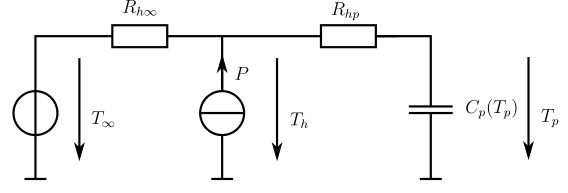
\includegraphics[width=12.5cm]{tikz/2_10_15_1b}
\end{figure}
\newline
Relevanten Größen:
\begin{align*}
	R_{h\infty} = \frac{1}{2r_o\pi L \alpha_\infty} \\
	C_p = r^2_i \pi L \rho_p c_{p,p}(T)
\end{align*}
und
\[
	R_{hp} = \frac{1}{2r_o\pi L k(r_o)}
\]
mit
\[
	k(r) = \frac{1}{r}\frac{1}{\frac{1}{\alpha_{hz}r_o} + \frac{1}{\lambda_z}\log\left( \frac{r_o}{r_i}\right) + \frac{1}{\alpha_{zp}r_i}}
\]
$k(r)$ wurde mit der Formel bei einer Wärmeleitung bei mehrschichtigen zylindrischen Wandaufbau aufgestellt.\\ \\
Einheiten:
\begin{align*}
	[R] &= KW^{-1} \\
	[C] &= JK^{-1} \\
	[P] &= W \\
	[T] &= K
\end{align*}
c) \\ \\
Die Differentialgleichung für die Ersatzschaltung lautet
\[
	\underbrace{(R_{hp} + R_{h\infty})C_p(T_p)}_{\tau(T_p)}\dot{T}_p = T_\infty + PR_{h\infty} - T_p
\]
Dadurch das $c_{p,p} = const$, wird die Differentialgleichung zu einer einfachen DGL 1.Ordnung.
Löst man diese erhält man die Lösung
\[
	T_p(t) = T_\infty + PR_{h\infty}(1 - exp(-t / \tau))
\]
	\newpage
\noindent
\textbf{Beispiel 2} \\ \\
a)\\ \\
Der Anteil durch die freie Konvektion lautet
\[
	\alpha_1(T_1)(T_1 - T_\infty)
\]
Mit der thermischen Strahlung  ergibt sich eine Leistung von
\[
	P = 2r_oL(\alpha_1(T_1)(T_1 - T_\infty) + \dot{q}_1)
\]
b) \\ \\
Dadurch das es sich bei den Oberflächen des Zylinders und des Maschinenbettes um konvexe Flächen handelt sind die Sichtfaktoren $F_{11}$ und $F_{22}$ gleich 0. Mit 
\[
	F_{11} + F_{12} + F_{1\infty} = 1
\]
und bekannten $F_{12}$ folgt
\[
	F_{1\infty} = 1 - F_{12}
\]
Aus dem Reziprozitätsgesetz schließt man
\begin{align*}
	CF_{21} = 2r_o\pi F_{12} \\
	F_{21} = \frac{2r_o\pi}{C}F_{12}
\end{align*}
Verwendet man das gleiche Gesetzt noch einmal an kann man daraus schließen das $F_{\infty1}$ und $F_{\infty2}$ gleich 0 ist, da $A_\infty \rightarrow \infty$. Mithilfe der Summationsregel kann man auf den Sichtfaktor $F_{\infty \infty}$ schlussfolgern, welcher den Wert 1 haben muss.\\ \\
c) \\ \\
Nettowärmestromdichte
\[
	\dot{\textbf{q}} = (\textbf{E} - \textbf{F})(\textbf{E} - (\textbf{E} - diag (\varepsilon))\textbf{F})^{-1}diag(\varepsilon)\sigma\textbf{T}^4
\]
mit
\[
	\dot{\textbf{q}} = [\dot{q}_1,\dot{q}_2,\dot{q}_\infty]^T , \textbf{T} = [T_1,T_2,T_\infty]^T, \varepsilon = [\varepsilon_1,\varepsilon_2,\varepsilon_\infty]^T
\]
der Einheitsmatrix \textbf{E} und dadurch das die Halle ein schwarzer Strahler ist, gilt
\[
	\varepsilon_\infty = 1
\]
Die Sichtfaktormatrix lautet
\[
	\textbf{F} = \begin{bmatrix}
	0 & F_{12} & F_{1\infty} \\
	F_{21} & 0 & F_{2\infty} \\
	0 & 0 & F_{\infty \infty}
	\end{bmatrix}
\]
	\newpage
\noindent
\textbf{Beispiel 3} \\ \\
Da für dieses Beispiel keine Musterlösung existiert, konnten leider keine Berechnungen durchgeführt werden, um diese dann anschließend mit der Musterlösung zu vergleichen. \\ \\
	\textbf{Beispiel 4} \\ \\
a) \\ \\
Aus der Zeichnung kann man direkt 
\[
	\textbf{p}_L = \begin{bmatrix}
		s + \sin\varphi \\
		- l \cos\varphi
	\end{bmatrix}
\]
ablesen. Um $\dot{\textbf{p}}_L$ zu bestimmen, muss man $\textbf{p}_L$ nach den Freiheitsgraden $s$ und $\varphi$ ableiten.\\
Geschwindigkeit der Lastposition
\[
	\dot{\textbf{p}}_L = \begin{bmatrix}
		\dot{s} + l\cos\varphi\dot{\varphi} \\
		l\sin\varphi\dot{\varphi}
	\end{bmatrix}
\]
Der Betrag dieses Vektors lautet
\[
	||\dot{\textbf{p}}_L||^2 = \dot{s}^2 + l^2\dot{\varphi}^2 + 2\dot{s}l\dot{\varphi}\cos\varphi
\]
Die kinetische Energie ergibt sich zu
\[
	T = \frac{1}{2} m_K \dot{s}^2 + \frac{1}{2}m_L||\dot{\textbf{p}}_L||^2 + \frac{1}{2} \Theta_{zz}\dot{\varphi}^2
\]
und die potentielle Energie
\[
	V = -m_lgl\cos\varphi + V_0
\]
mit 
\[
	V_0 = m_Lgl
\]
zu
\[
	V = m_Lgl(1 - \cos\varphi) 
\]
b) \\ \\
Um die Bewegungsgleichungen zu bestimmen wird als erstes die Lagrange-Funktion benötigt welche lautet
\begin{align*}
	L &= T - V = \frac{1}{2} m_K \dot{s}^2 + \frac{1}{2}m_L||\dot{\textbf{p}}_L||^2 + \frac{1}{2} \Theta_{zz}\dot{\varphi}^2 - m_Lgl(1 - \cos\varphi) \\
	&=  \frac{1}{2} m_K \dot{s}^2 + \frac{1}{2}m_L (\dot{s}^2 + l^2\dot{\varphi}^2 + 2\dot{s}l\dot{\varphi}\cos\varphi)  + \frac{1}{2} \Theta_{zz}\dot{\varphi}^2 - m_Lgl(1 - \cos\varphi)
\end{align*}
Euler-Lagrange-Formalismus
\[
	\frac{d}{dt}\frac{\partial L}{\partial \dot{\textbf{q}}} - \frac{\partial L}{\partial \textbf{q}} = \textbf{f}_{np}
\]
\newpage
\noindent
Die seperaten Ableitungen
\begin{align*}
	\frac{\partial L}{\partial \textbf{q}} &= \begin{bmatrix}
		0 \\
		-m_Ll\sin\varphi(\dot{s}\dot{\varphi} + g)
	\end{bmatrix}
	\\
	\frac{\partial L}{\partial \dot{\textbf{q}}} &= \begin{bmatrix}
		(m_K + m_L)\dot{s} + m_Ll\dot{\varphi}\cos\varphi \\
		(\Theta_{zz} + m_L)\dot{\varphi} + m_Ll\dot{s}\cos\varphi
	\end{bmatrix}
	\\
	\frac{d}{dt}\frac{\partial L}{\partial \dot{\textbf{q}}} &= \begin{bmatrix}
		(m_k + m_L)\ddot{s} + m_Ll\ddot{\varphi}\cos\varphi - m_Ll\dot{\varphi}^2\sin\varphi \\
		(\Theta_{zz} + m_L)\ddot{\varphi} + m_Ll\ddot{s}\cos\varphi - m_Ll\dot{s}^2\sin\varphi
	\end{bmatrix}
\end{align*}
Die externen Kräfte können direkt aus der Angabe ablesen werden und lauten
\[
	\textbf{f}_{np} = \begin{bmatrix}
		-d_K\dot{s} + F \\ 
		0
	\end{bmatrix}
\]
c) \\ \\
Aus der zweiten Zeile der Bewegungsgleichungen aus Punkt b) erhält man die Bewegungsgleichung der haftenden Laufkatze. Dadurch lautet diese
\[
	(\Theta_{zz} + m_L)\ddot{\varphi} + m_Llg\sin\varphi = 0
\]
d) \\ \\
Als erstes müssen die externen Kräfte um die Haftkraft $F_H$ erweitert werden. Daher lauten diese dann
\[
	\textbf{f}_{np} = \begin{bmatrix}
	-d_K\dot{s} + F + F_H\\ 
	0
	\end{bmatrix}
\]
Betrachtet man laut Hinweis nur die erste Zeile der Bewegungsgleichungen aus Punkt b) mit $\dot{s} = \ddot{s} = 0$ erhält man
\[
	m_Ll\ddot{\varphi}\cos\varphi - m_Ll\dot{\varphi}^2\sin\varphi = F + F_H
\] 
Formt nun auf $F_H$ um und ermittelt man den Betrag erhält man
\[
	|F_H| = |m_Ll\ddot{\varphi}\cos\varphi - m_Ll\dot{\varphi}^2\sin\varphi - F|
\]
Bringt man nun schließlich diese Gleichung auf die Form der Haftreibung erhält man schlussendlich die Haftbedingung
\[
	|F_H| = |m_Ll\ddot{\varphi}\cos\varphi - m_Ll\dot{\varphi}^2\sin\varphi - F| \leq \mu F_N
\]
Mit
\[
	\ddot{\varphi} = - \frac{m_Llg\sin\varphi}{\Theta_{zz} + m_Ll^2}
\]
aus Punkt c), erhält man die vereinfachte Haftbedingung
\begin{align*}
	\biggl|m_Ll\frac{m_Llg\sin\varphi}{\Theta_{zz} + m_Ll^2}\cos\varphi - m_Ll\dot{\varphi}^2\sin\varphi - F\biggl| \leq \mu F_N \\ \\
	\biggl|\frac{gm^2_Ll^2\sin\varphi\cos\varphi}{\Theta_{zz} + m_Ll^2} + m_Ll\dot{\varphi}^2\sin\varphi + F\biggl| \leq \mu F_N
\end{align*}
	
	\newpage
	\subsection{27.11.2015}
	\textbf{Beispiel 1} \\ \\
a)\\ \\
Um das Bremsmoment ermitteln zu können benötigt man zu aller erst einmal die Wirkfläche. In diesem  Beispiel beträgt diese Fläche
\[
	A = \int_{R_i}^{R_a}\int_{0}^{\frac{\pi}{3}}rd\varphi dr = \frac{\pi}{6}\left(R_a^2 - R_i^2\right)
\]
Das Bremsmoment lässt sich mit 
\[
	M_R = \int_{R_i}^{R_a}\int_{0}^{\frac{\pi}{3}} r^2\mu\frac{F_B}{A}d\varphi dr
\]
zu 
\begin{align*}
	M_R &= \int_{R_i}^{R_a}\int_{0}^{\frac{\pi}{3}} r^2\mu F_B \frac{6}{\pi \left(R_a^2 - R_i^2\right)}d\varphi dr = \\
	M_R &= \int_{R_i}^{R_a} r^2 \mu F_B \frac{\cancelto{2}{6}}{\cancel{\pi} \left(R_a^2 - R_i^2\right)} \frac{\cancel{\pi}}{\cancel{3}} dr = \\
	M_R &= \mu F_B \frac{2}{3}\frac{R_a^3 - R_i^3}{R_a^2 - R_i^2}
\end{align*}
Da zwei Bremsbacken zum Abbremsen verwendet werden lautet das gesamte Bremsmoment 
\[
	M_{ges} = 2M_R = \mu F_B \frac{4}{3}\frac{R_a^3 - R_i^3}{R_a^2 - R_i^2}
\]
b) \\ \\
Die Bewegungsdifferenzialgleichung der Schwungscheibe lautet
\[
	\ddot{\varphi} = - \frac{M_{ges}}{\Theta_{zz}}
\]
Das "$-$" vor dem Brauch kommt daher, dass die $\ddot{\varphi}$ mit der Zeit immer kleiner werden soll, da ja ein Bremsvorgang stattfindet.
Die Anfangsbedingungen für dieses Problem lauten
\[
	\varphi(0) = 0
\]
kann aber beliebig gewählt werden, und 
\[
	\omega(0) = \overline{\omega}
\]
\newpage
\noindent
Als nächstes muss man diese Differenzialgleichung lösen. Dies erreicht man durch 2-maliges Integrieren.
\begin{align*}
	\omega(t) = \dot{\varphi}(t) &= - \frac{M_{ges}}{\Theta_{zz}}t + \overline{\omega} \\
	\varphi(t) &= - \frac{M_{ges}}{\Theta_{zz}} \frac{t^2}{2} + \overline{\omega}t
\end{align*}
Damit ergibt sich die Bremsdauer $t_B$ zu
\begin{align*}
	0 &= \overline{\omega} - \frac{M_{ges}}{\Theta_{zz}}t_B \\ 
	\overline{\omega} &= \frac{M_{ges}}{\Theta_{zz}}t_B \\
	t_B &= \frac{\Theta_{zz}\overline{\omega}}{M_{ges}}
\end{align*}
Um die Bremskraft $F_B$ zu bestimmen setzt man $M_{ges}$ ein und formt einfach auf $F_H$ um und man erhält
\[
	F_B = \frac{3}{4}\frac{R_a^2 - R_i^2}{R_a^3 - R_i^3}\frac{\Theta_{zz}\overline{\omega}}{t_B\mu}
\]
c) \\ \\
Die Bremsleistung lässt sich mit $\dot{W}_R = -M_{ges}\omega$ ermitteln. In diesem Fall lautet somit die Bremsleistung
\[
	\dot{W}_R = \frac{M_{ges}^2}{\Theta_{zz}}t - M_{ges}\overline{\omega}
\]
Integriert man nun diese Leistung über die Bremsdauer erhält man die Energie
\begin{align*}
	E_B &= \int_{0}^{t_B}\frac{M_{ges}^2}{\Theta_{zz}}t - M_{ges}\overline{\omega} dt = \\
	&= \frac{1}{2}\frac{M_{ges}^2}{\Theta_{zz}}\frac{\Theta_{zz}^2\overline{\omega}^2}{M_{ges}^2} - M_{ges}\overline{\omega}\frac{\Theta_{zz}\overline{\omega}}{M_{ges}} \\
	&= -\frac{1}{2}\Theta_{zz}\overline{\omega}
\end{align*}
Dies entspricht der im Schwungrad gespeicherten Energie.\\ \\
d) \\ \\
Aus dem ersten Hauptsatz der Thermodynamik ergibt sich die Differenzialgleichung 
\[
	m_Bc_B\frac{dT_B(t)}{dt} = \frac{1}{2}\left(M_{ges}\overline{\omega} - \frac{M_{ges}^2}{\Theta_{zz}}t\right)
\]
Löst man diese Gleichung durch einfaches Integrieren erhält man
\begin{align*}
	T_B(t) = \frac{1}{2m_Bc_B}\left(M_{ges}\overline{\omega}t - \frac{1}{2}\frac{M_{ges}^2}{\Theta_{zz}}t^2\right) + C
\end{align*}
Setzt man die AB $T_B(0) = T_{B,0}$ ein erhält man
\[
	T_B(t) = T_{B,0} + \frac{1}{2m_Bc_B}\left(M_{ges}\overline{\omega}t - \frac{1}{2}\frac{M_{ges}^2}{\Theta_{zz}}t^2\right)
\]
Zum Zeitpunkt $t_B$ ergibt sich nun folgende Temperatur
\begin{align*}
		T_B(t) &= T_{B,0} + \frac{1}{2m_Bc_B}\left(M_{ges}\overline{\omega}t_B - \frac{1}{2}\frac{M_{ges}^2}{\Theta_{zz}}t_B^2\right) = \\
		&= T_{B,0} + \frac{\Theta_{zz}\overline{\omega}^2}{4m_Bc_B} = \\
		&= T_{B,0} - \frac{1}{m_Bc_B}\frac{E_B}{2} 
\end{align*}
	\textbf{Beispiel 2} \\ \\
Die Wärmestromdichte $\dot{q}_{1-\infty}^I$ ohne der Rettungsdecke lässt sich mit der Formel für die Wärmestromdiche bei Konvektion bestimmen. Diese lautet
\[
	\dot{q}_{1-\infty}^I = \varepsilon_1\sigma(T_1^4 - T_\infty^4)
\]
Um den Wärmestrom zu erhalten muss die Wärmestromdichte einfach mit der betreffenden Fläche multipliziert werden.
\[
	Q_{1-\infty}^I = \varepsilon_1A_1\sigma(T_1^4 - T_\infty^4)
\]
Die Sichtfaktormatrix für dieses Wärmeproblem lautet
\begin{align*}
	\textbf{F} = \begin{bmatrix}
		0 & 1 \\
		1 & 0	
	\end{bmatrix}
	\\
	diag(\varepsilon) = \begin{bmatrix}
		\varepsilon_1 & 0 \\
		0 & \varepsilon_2
	\end{bmatrix}
\end{align*}
Mit der Formel für die Nettowärmestromdichte kann der Wärmestrom zwischen den beiden Körpern bestimmt werden zu
\[
	Q_{1-2}^{II} = \sigma A_1 \frac{\varepsilon_1 \varepsilon_2}{\underbrace{1 - (1 - \varepsilon_1)(1 - \varepsilon_2)}_{K}}(T_1^4 - T_2^4 )
\]
Der Wärmestrom zwischen Rettungsdecke und Umgebung lautet
\[
	Q_{2-\infty}^{II} = \varepsilon_2 A_1\sigma(T_2^4 - T_\infty^4)
\]
Da $Q_{1-2}^{II} = Q_{2-\infty}^{II}$ gilt, kann man $T_2^4$ bestimmen zu
\[
	T_2^4 = \frac{K}{K + \varepsilon_2}T_1^4 + \frac{\varepsilon_2}{K + \varepsilon_2}T_\infty^4
\]
Setzt man dies nun in $Q_{1-2}^{II}$ ein erhält man
\[
	Q_{1-2}^{II} = \sigma A_1 \frac{K\varepsilon_2}{K + \varepsilon_2}(T_1^4 - T_\infty^4)
\]
welcher mit $Q_{1-\infty}^{II}$ gleichzusetzen ist.
Nun kann man das Verhältnis zwischen den Wärmeströmen mit und ohne Decke bestimmen und man erhält ein Verhältnis von $2/5$. Daraus kann man schließen, dass durch die Decke $3/5$ weniger Wärme an die Umgebung verloren geht.
	\\ \\
\textbf{Beispiel 3} \\ \\
a)\\ \\
Zur Beschreibung der Bewegung des Schlittens reicht ein einziger Freiheitsgrad aus, da sich sich dieser nur in horizontaler Richtung bewegt. Die geeignete Minimalkoordinate lautet
\[
	q = \varphi_1(t)
\]
b) \\ \\
Die Kniehebelpresse muss folgende Zwangsbedingung erfüllen.
\[
	L_1\sin\varphi_1 - L_2\sin\varphi_2 = 0
\]
Aus dieser kann nun leicht $\varphi_2$ bestimmen.
\begin{align*}
	L_1\sin\varphi_1 - L_2\sin\varphi_2 = 0  \\
	L_2\sin\varphi_2 = L_1\sin\varphi_1 \\
	\varphi_2 = \arcsin\left(\frac{L_1}{L_2}\sin\varphi_1\right)
\end{align*}
c) \\ \\
Die Ortsvektoren können direkt aus der Angabe abgelesen werden.
\begin{align*}
	\textbf{r}_1 &= \frac{L_1}{2}\begin{bmatrix}
		\cos(q) \\
		\sin(q)
	\end{bmatrix} 
	\\
	\textbf{r}_2 &= L_1\begin{bmatrix}
	\cos(q) \\
	\sin(q)
	\end{bmatrix} 
	+ 
	\frac{L_2}{2}\begin{bmatrix}
		\cos(\varphi_2(q)) \\
		-\sin(\varphi_2(q))
	\end{bmatrix}
\end{align*}
d) \\ \\
Die Schwerpunktsgeschwindigkeiten der Schenkel lauten
\begin{align*}
	\textbf{v}_1 &= \frac{L_1}{2}\begin{bmatrix}
		-\sin(q) \\
		 \cos(q)
	\end{bmatrix} \dot{q}
	\\
	\textbf{v}_2 &= L_1 \begin{bmatrix}
	-\sin(q) \\
	\cos(q)
	\end{bmatrix} \dot{q}
	+
	\frac{L_2}{2}\begin{bmatrix}
		-\sin(\varphi_2(q)) \\
		-\cos(\varphi_2(q))
	\end{bmatrix}
	\frac{\partial \varphi_2(q)}{\partial q} \dot{q}
\end{align*}
Die Drehwinkelgeschwindigkeiten lauten
\begin{align*}
	\omega_1 &= \dot{q} \\
	\omega_2 &= - \frac{\partial \varphi_2(q)}{\partial q} \dot{q}
\end{align*}
e) \\ \\
Anfangs müssen einige Zwischenrechnungen durchgeführt werden.
\begin{align*}
	v_1^2 &= \frac{L_1^2}{4}\dot{q}^2(\cos^2(q) + \sin^2(q)) \\
		  &= \frac{L_1^2}{4}\dot{q}^2
\end{align*}
\begin{align*}
	v_2^2 &= \left(-L_1\sin(q)\dot{q} - \frac{L_2}{2}\sin(\varphi_2(q))\frac{\partial \varphi_2(q)}{\partial q}\dot{q}\right)^2 + \left(L_1\cos(q)\dot{q} - \frac{L_2}{2}\cos(\varphi_2(q))\frac{\partial \varphi_2(q)}{\partial q}\dot{q}\right)^2 \\
	&= L_1^2\dot{q}^2\sin^2(q) + L_1L_2\dot{q}^2\sin(q)\sin(\varphi_2(q))\frac{\partial \varphi_2(q)}{\partial q} + \frac{L_2^2}{4}\dot{q}^2\left(\frac{\partial \varphi_2(q)}{\partial q}\right)^2\sin^2(\varphi_2(q)) + \\
	&+ L_1^2\dot{q}^2\cos^2(q) - L_1L_2\dot{q}^2\cos(q)\cos(\varphi_2(q))\frac{\partial \varphi_2(q)}{\partial q} + \frac{L_2^2}{4}\dot{q}^2\left(\frac{\partial \varphi_2(q)}{\partial q}\right)^2\cos^2(\varphi_2(q)) \\
	&= L_1^2\dot{q}^2 + \frac{L_2^2}{4}\dot{q}^2\left(\frac{\partial \varphi_2(q)}{\partial q}\right)^2 - L_1L_2\dot{q}^2\frac{\partial \varphi_2(q)}{\partial q}(\cos(q)\cos(\varphi_2(q)) - \sin(q)\sin(\varphi_2(q))) \\
	&= L_1^2\dot{q}^2 + \frac{L_2^2}{4}\dot{q}^2\left(\frac{\partial \varphi_2(q)}{\partial q}\right)^2 - L_1L_2\dot{q}^2\frac{\partial \varphi_2(q)}{\partial q}\cos(q + \varphi_2(q))
\end{align*}
Die kinetische Energie lässt sich mit den Formeln aus der Formelsammlung bestimmen und lautet daher:
\begin{align*}
	T &= \frac{1}{2} m_1v_1^2 + \frac{1}{2}m_2v_2^2 + \frac{1}{2} \Theta_1 \omega_1^2 + \frac{1}{2}\Theta_2\omega_2^2 \\
	&= \frac{1}{8}m_1L_1^2\dot{q}^2 + \frac{1}{2}m_2L_1^2\dot{q}^2 + \frac{1}{8}m_2L_2^2\left(\frac{\partial \varphi_2(q)}{\partial q}\right)^2\dot{q}^2 - \frac{1}{2}m_2L_1L_2\cos(q + \varphi_2(q))\left(\frac{\partial \varphi_2(q)}{\partial q}\right)\dot{q}^2 + \\
	&+ \frac{1}{2}\Theta_1\dot{q}^2 + \frac{1}{2}\Theta_2\left(\frac{\partial \varphi_2(q)}{\partial q}\dot{q}\right)^2
\end{align*}
f) \\ \\
Die potenzielle Energie der Schenkel zufolge der Schwerkraft lautet
\begin{align*}
	V_q &= \frac{1}{2}m_1gL_1\sin(q) + m_2gL_1\sin(q) - \frac{1}{2}m_2gL_2\sin(\varphi_2(q)) \\
	V_F  &= \frac{1}{2}c_F\left(L_1\cos(q) + \frac{1}{2}L_2\cos(\varphi_2(q)) - x_{F,0}\right)^2
\end{align*}
\newpage
\noindent
g) \\ \\
Angriffspunkte der beiden externen Kräfte:
\begin{align*}
	\textbf{r}_F &= L_1\begin{bmatrix}
		\cos(q) \\
		\sin(q)
	\end{bmatrix}
	\\
	\textbf{r}_{F_L} &= L_1\begin{bmatrix}
	\cos(q) \\
	\sin(q)
	\end{bmatrix}
	+
	L_2 \begin{bmatrix}
		\cos(\varphi_2(q)) \\
		-\sin(\varphi_2(q))
	\end{bmatrix}
\end{align*}
Deren Ableitungen nach der generalisierten Koordinate lautet
\begin{align*}
	\frac{\partial \textbf{r}_F}{\partial q} &= L_1 \begin{bmatrix}
		-\sin(q) \\
		\cos(q)
	\end{bmatrix}
	\\
	\frac{\partial \textbf{r}_{F_L}}{\partial q} &= L_1\begin{bmatrix}
	-\sin(q) \\
	\cos(q)
	\end{bmatrix}
	+
	L_2\begin{bmatrix}
	-\sin(\varphi_2(q)) \\
	-\cos(\varphi_2(q))
	\end{bmatrix}
	\frac{\partial \varphi_2(q)}{\partial q}
\end{align*}
Die Vektoren der externen Kräfte lauten hier
\begin{align*}
	\textbf{F} &= \begin{bmatrix}
	0 \\
	- F
	\end{bmatrix}
	\\
	\textbf{F}_L &= \begin{bmatrix}
		-F_L \\
		0
	\end{bmatrix}
\end{align*}
Mit der Formel für die generalisierten Kräfte aus der Formelsammlung diese folgendermaßen aussehen.
\begin{align*}
	f_F &= \textbf{F}^T\frac{\partial \textbf{r}_F}{\partial q} = -FL_1\cos(q) \\
	f_{F_L} &= \textbf{F}_L^T \frac{\partial \textbf{r}_{F_L}}{\partial q} = F_L \left(L_1\sin(q) + L_2\sin(\varphi_2(q))\frac{\partial \varphi_2(q)}{\partial q}\right)
\end{align*}
	
	\newpage
	\subsection{05.02.2016}
	\textbf{Beispiel 1} \\ \\
Bei diesen Beispiel muss man den physikalischen Hintergrund von Seilrollen genau beachten. \\ \\
a)\\ \\
Um die kinetische Energie T zu bestimmen, benötigt man sämtliche im System auftretenden Geschwindigkeiten.
\begin{align*}
	\omega_{R_1} &= \frac{v}{r_1} \\
	v_{R_2} &= v \frac{r_1}{2r_2} \\
	\omega_{R_2} &= v\frac{r_1}{2r_2^2}
\end{align*}
Somit ergibt sich die kinetische Energie zu
\[
	T = \frac{m_Lv^2}{2} + \frac{\Theta_1\omega_{R_1}^2}{2} + \frac{\Theta_2\omega_{R_2}^2}{2} + \frac{m_2v_{R_2}^2}{2}
\]
b) \\ \\
Die Energie 
\[
	W = F \cdot s
\]
die beim Verschieben benötigt wird lautet
\[
	W = \mu_cm_Lg\cos\phi s
\]
c) \\ \\
Zum Zeitpunkt $t_0$ soll
\[
	V(t_0) = 0
\]
gültig sein.
Zum Zeitpunkt $t_1$ sieht die potentielle Energie folgendermaßen aus
\[
	V(t_1) = m_Lgs\sin\phi - m_2g\frac{r_1}{2r_2}
\]
d) \\ \\
Die aufzuwendende Arbeit durch die Kraft $\textbf{F}$ lautet
\[
	W = Fs\frac{r_1}{2r_2}
\]
e) \\ \\
Aus der Energieerhaltung ergibt sich
\[
	T(t_0) + V(t_0) + W_F - W = T(t_1) + V(t_1)
\]
Bei den Termen mit $t_0$ müssen für $v$ und $\omega$, $v_0$ und $\omega(t_0)$ und bei $t_1$, $v_1$ und $\omega(t_1)$ eingesetzt werden. Schreibt man nun die obige Gleichung komplett aus und formt dieses dann auf die gesuchte Kraft um erhält man
\begin{align*}
	F &=  \frac{2r_2}{sr_1}\left( m_L\frac{v_1^2 - v_0^2}{2} + \Theta_1 \frac{\omega_{R_1}(t_1)^2 - \omega_{R_1}(t_0)^2}{2} + \Theta_2 \frac{\omega_{R_2}(t_1)^2 - \omega_{R_2}(t_0)^2}{2}\right) + \\
	&+\frac{2r_2}{sr_1}  \left(m_2\frac{v_{R_2}(t_1)^2 - v_{R_2}(t_0)^2}{2} + m_Lgs(\sin\phi + \mu_c\cos\phi) - m_2gs\frac{r_1}{2r_2}\right)
\end{align*}
	\subsection{11.03.2016}
	\subsection{13.05.2016}
	\subsection{08.07.2016}
	\subsection{23.06.2016}
	\subsection{18.11.2016}
	\subsection{03.02.2017}
	\subsection{31.03.2017}
	\subsection{19.05.2017}
	\subsection{14.07.2017}
	\subsection{29.09.2017}
	\subsection{01.12.2017}
	\subsection{02.02.2018}
	\subsection{16.03.2018}
	\subsection{18.05.2018}
	\subsection{13.07.2018}
	\subsection{28.09.2018}
	\subsection{30.11.2018}
	\subsection{01.02.2019}
	
	\newpage
	\subsection{15.03.2019}
	%\documentclass{article}
%\usepackage{tikz}
%\usepackage{amsmath}
%\begin{document}
\noindent
\textbf{Beispiel 1} \\ \\
a) 
	\begin{figure}[h]
		\centering
		\usetikzlibrary{arrows}
\tikzset{
pil/.style={
	->,thick,
	shorten<=2pt,
	shorten>=2pt,}
}
\begin{tikzpicture}[scale=0.75]
\draw (-5,0)--(5,0); %Grundfläche
\draw(-4.5,-0.075)--(-4.25,-0.75)--(-4,-0.075)--(-4.5,-0.075); %Gleitlager
\draw [fill=white]  (-4.25,-0.75) circle [radius=5pt];
\draw(4.5,0)--(4.25,-0.75)--(4,0); %Festlager
\draw [fill=white]  (4.25,-0.75) circle [radius=5pt];

\draw [fill=white] (-3,0) rectangle (3,3);
%Kräfte
\draw [->](0,2)--(0,1);
\draw (0.25,1.5) node {\(f_g\)};
\draw [<-](-4.25,-1.25) -- (-4.25,-2.25);
\draw  (-3.75,-2) node {\(f_{A,y}\)};
\draw [<-](4.25,-1.25) -- (4.25,-2.25);
\draw  (4.8,-1.85) node {\(f_{B,y}\)};
\draw [<-](4.75,-0.75) -- (5.75,-0.75);
\draw  (5.25,-0.5) node {\(f_{B,x}\)};
%\draw [fill=blue] (0,0) arc [start angle=90,end angle=300, radius=10pt];
%\draw  [fill=blue] (0,0) -- (2,0.5);



\end{tikzpicture}
	\end{figure} \\
%\noindent
Um die Kräfte in den Lagern zu bestimmten, stellen wir zuerst das Kräftegleichgewicht und die Momenten Gleichung im Punkt B auf. 
\begin{align*}\label{key}
x&: 0=f_{B,x} \\
y&: 0 = f_A + f_{B,y} -f_g\\
M_B&:0=b f_g-2L \cos(\alpha)  
\end{align*}

\noindent
Formt man nun die Momenten Gleichung nach \(f_A\) um folgt: 
\begin{align*}
f_A = \frac{b f_g}{2L \cos(\alpha)} \qquad f_{B_x}=0 \qquad f_{B,y} = \left(1-\frac{b}{2L \cos(\alpha)}\right) f_g
\end{align*}
\begin{figure}[h]
	\centering
	\begin{tikzpicture}[scale=0.5]

\node (v1) at (-2.5,-2.5) {};
\node (v2) at (2.5,2.5) {};
\node (v3) at (0,0) {};
\node (v4) at (-2.5,2.5) {};
\node (v5) at (2.5,-2.5) {};
\draw  (v1) circle (0.2);
\draw  (v2) circle (0.2);
\draw  (v3) circle (0.2);
\draw  (v4) circle (0.2);
\draw  (v5) circle (0.2);
\draw (-2.9,-2.2) -- (2.1,2.8);
\draw (-2.2,-2.9) -- (2.9,2.2);
\draw (-2.117,-2.8214) arc (-40.0022:-230:0.5);
\draw (2.117,2.8214) arc (139.9978:-40:0.5);
\draw (2,2.7) -- (2.2,2.9);
\draw[black!50] (-1.8,-2.5) -- (1.5,-2.5);

\draw (-0.6,-2.5) arc (0:19:3.1);
\draw  (-1,-2.1) node {\(\alpha\)};
\draw (-2.8,2.1) -- (2.1,-2.8);
\draw (-2.1,2.8) -- (2.9,-2.2);
\draw (2.117,-2.8214) arc (-139.9978:40:0.5);
\draw (-2.75,2.067) arc (-120.0007:-325:0.5);
\draw [->](0,-0.3) -- (0,-1.4) ;
\draw (1.2,-1.4) node {\(m_2 g\)};
\draw[<-] (2.5,-3.2) -- (2.5,-4.1);
\draw (3.5,-3.6) node {\(f_{E,y}\)};
\draw [<-](-2.5,-3.2) -- (-2.5,-4);
\draw (-1.5,-3.6) node {\(f_{D_y}\)};
\draw[<-] (2.5,3.2) -- (2.5,4.1);
\draw (3.5,3.6) node {\(f_{B,y}\)};
\draw [<-](-2.5,3.2) -- (-2.5,4);
\draw (-1.5,3.6) node {\(f_{A_y}\)};

\end{tikzpicture}
\end{figure}
b) \\
%\noindent
Um die Kräfte in den Punkten D und E zu bestimmen, stellen wir das Kräftegleichgewicht in den Trägern auf, daraus folgt: 
\begin{align*}
 f_{D,y} = m2 g + f_{B,y}\qquad	f_{E,y} = m_2 g + f_A 
\end{align*}

\begin{figure}[h]
	\centering
	\begin{tikzpicture}[scale=0.5]

\node (v1) at (-2.5,-2.5) {};
\node (v2) at (2.5,2.5) {};
\node (v3) at (0,0) {};
%\node (v4) at (-2.5,2.5) {};
%\node (v5) at (2.5,-2.5) {};
\draw  (v1) circle (0.2);
\draw  (v2) circle (0.2);
\draw  (v3) circle (0.2);
%\draw  (v4) circle (0.2);
%\draw  (v5) circle (0.2);
\draw (-2.9,-2.2) -- (2.1,2.8);
\draw (-2.2,-2.9) -- (2.9,2.2);
\draw (-2.117,-2.8214) arc (-40.0022:-230:0.5);
\draw (2.117,2.8214) arc (139.9978:-40:0.5);
\draw (2,2.7) -- (2.2,2.9);
\draw[black!50] (-1.8,-2.5) -- (1.5,-2.5);

\draw (-0.6,-2.5) arc (0:19:3.1);
\draw  (-1,-2.1) node {\(\alpha\)};
% \draw (-2.8,2.1) -- (2.1,-2.8);
% \draw (-2.1,2.8) -- (2.9,-2.2);
% \draw (2.117,-2.8214) arc (-139.9978:40:0.5);
% \draw (-2.75,2.067) arc (-120.0007:-325:0.5);
\draw [->](0,-0.3) -- (0,-1.4) ;
\draw (0.8,-1.0) node {\(m_2 g\)};
% \draw[<-] (2.5,-3.2) -- (2.5,-4.1);
% \draw (3,-3.6) node {\(f_{D,y}\)};
\draw [<-](-2.5,-3.2) -- (-2.5,-4);
\draw (-1.5,-3.6) node {\(f_{D_y}\)};
\draw[<-] (2.5,3.2) -- (2.5,4.1);
\draw (3.5,3.6) node {\(f_{B,y}\)};
% \draw [<-](-2.5,3.2) -- (-2.5,4);
%\draw (-2.0,3.6) node {\(f_{A_y}\)};



\draw [<-](-3.3,-2.5) -- (-4.2,-2.5);
\draw (-3.7,-3.2) node {\(f_{D,x}\)};
\draw [<-](3.3,2.5) -- (4.2,2.5);
\draw (3.7,1.7) node {\(f_{B,x}\)};
\end{tikzpicture}
\end{figure}
\noindent
c)\\  \\ %\noindent
Um die Kräfte in den Lagern D und E in horizontaler (x-Richtung) zu bestimmen schneiden wir die Hubstangen getrennt voneinander frei und stellen die Kraftgleichungen und die Momenten Gleichung auf. 

\begin{align*}
	x&:  0 = f_{E,x} - f_{D,x}\\
	y&:  \text{wurde bereits bestimmt} \\ 
	M_D&: 0 = m_2 g \cos(\alpha) +f_{B,x} \sin(\alpha) + f_{B,y} \cos(\alpha)
\end{align*}
Aus der Momenten Gleichung  folgt: 
\begin{align*}
	f_{B,x} = \frac{m_2 g- f_{B,y}}{\tan{\alpha}} =f_{E,x} \qquad  F(\alpha) = f_{D,x} = -f_{E,x}
\end{align*}
\noindent 
d) \\ \\ 	
	Um die Haftbedingung zu berechnen formt man \(F(\alpha) = \mu_H f_{D,y}\) um und setzt für \(\alpha=\frac{\pi}{4}\) ein: 
	
	\begin{align*}
		\mu_H \geq \frac{F(\alpha)}{f_{D,y}} = \frac{m_1+m_2}{m_2+\frac{m_1 b}{\sqrt2L}}
	\end{align*}
	
%\end{document}	
	\newpage
\noindent
\textbf{Beispiel 2} \\ \\
a) \\ \\
%\noindent
Die Oberfläche des Öl's strahlt nicht auf sich selbst, deshalb lautet der Sichtfaktor Matrixeintrag \(F_{OO} = 0\), aus der Summationsregel folgt \(F_{OH} = 1 - F_{OO} = 1\). Aus dem Reziprozitätsgesetz folgt \(F_{HO}=\frac{A_O}{A_H}F_{OH} \). Der Letzte Eintrag lautet wegen der Summationsregel \(F_{HH}=1-\frac{A_O}{A_H}\)

\[\textbf{F}=\left[\begin{matrix}
0 & 1 \\ \frac{A_O}{A_H} & 1 -\frac{A_O}{A_H} \end{matrix}\right]\]

\begin{tiny}
%\hspace{100px}	
\( \hspace{-75pt}\dot{\textbf{q}}=  \left[ \begin {array}{c} \sigma\, \left(  \left( {\frac {\varepsilon_
		{H}\,A_{H}-\varepsilon_{H}\,A_{O}+A_{O}}{-A_{O}\,\varepsilon_{H}\,
		\varepsilon_{O}+\varepsilon_{H}\,A_{H}+A_{O}\,\varepsilon_{O}}}+{
	\frac { \left( -1+\varepsilon_{H} \right) A_{O}}{-A_{O}\,\varepsilon_{
			H}\,\varepsilon_{O}+\varepsilon_{H}\,A_{H}+A_{O}\,\varepsilon_{O}}}
\right) \varepsilon_{O}\,{{\it TO}}^{4}+ \left( -{\frac { \left( -1+
		\varepsilon_{O} \right) A_{H}}{-A_{O}\,\varepsilon_{H}\,\varepsilon_{O
		}+\varepsilon_{H}\,A_{H}+A_{O}\,\varepsilon_{O}}}-{\frac {A_{H}}{-A_{O
		}\,\varepsilon_{H}\,\varepsilon_{O}+\varepsilon_{H}\,A_{H}+A_{O}\,
		\varepsilon_{O}}} \right) \varepsilon_{H}\,{{\it TH}}^{4} \right) 
\\ \noalign{\medskip}\sigma\, \left(  \left( -{\frac {A_{O}\, \left( 
		\varepsilon_{H}\,A_{H}-\varepsilon_{H}\,A_{O}+A_{O} \right) }{A_{H}\,
		\left( -A_{O}\,\varepsilon_{H}\,\varepsilon_{O}+\varepsilon_{H}\,A_{H
		}+A_{O}\,\varepsilon_{O} \right) }}-{\frac {{A_{O}}^{2} \left( -1+
		\varepsilon_{H} \right) }{A_{H}\, \left( -A_{O}\,\varepsilon_{H}\,
		\varepsilon_{O}+\varepsilon_{H}\,A_{H}+A_{O}\,\varepsilon_{O} \right) 
}} \right) \varepsilon_{O}\,{{\it TO}}^{4}+ \left( {\frac {A_{O}\,
		\left( -1+\varepsilon_{O} \right) }{-A_{O}\,\varepsilon_{H}\,
		\varepsilon_{O}+\varepsilon_{H}\,A_{H}+A_{O}\,\varepsilon_{O}}}+{
	\frac {A_{O}}{-A_{O}\,\varepsilon_{H}\,\varepsilon_{O}+\varepsilon_{H}
		\,A_{H}+A_{O}\,\varepsilon_{O}}} \right) \varepsilon_{H}\,{{\it TH}}^{
	4} \right) \end {array} \right] 
\)
\end{tiny}
\\ \newline
\bigskip
\noindent
Um diesen Vektor zu ermitteln, wird einfach der Formalismus der Nettowärmestromdichte genutzt.
Der Vektor \(\dot{\textbf{q}}\) besteht aus den Einträgen \(\dot{q}_O\) und \(\dot{q}_H\), wir benötigen aber nur den ersten Eintrag, weil \(\dot{Q}_{rad} = A_O \dot{q}_O\) lautet.
\bigskip \\
b) \\
\\
Um die stationäre thermische Energiebilanz zu bestimmen müssen alle Wärmeströme die ein- oder austreten addiert werden. 

\[\dot{m}_{LM} c_{p,LM} (T_\infty-T_L)+0.2\dot{m}_{LM} c_{p,O}-A_O \alpha_{OL}(T_O-T_\infty)-\dot{Q}_{rad}+P_{el}\eta=0\]
\bigskip 

\noindent c)  \\ 
\\ 
Die Temperatur \(T_O\) lautet nun \(\overline{T}_O\) und wird in die Lösung von b eingesetzt. Danach muss die Gleichung nach \(P_{el}\) umgeformt werden. Daraus ergibt sich. 

\[P_{el}=\frac{1}{\eta}\left(-\dot{m}_{LM} c_{p,LM} (T_\infty-T_L)-0.2\dot{m}_{LM} c_{p,O}-A_O \alpha_{OL}(T_O-T_\infty)+\dot{Q}_{rad}\right)\]

\bigskip 

\noindent d)  \\ 
\\
Die Anfangsbedienung der Differentialgleichung lautet \(T_O(t=0)=\overline{T}_O\) und die Differentialgleichung erhält man indem man die Fouriersche Wärmeleitgleichung nach dem Volumen integriert. Zu beachten ist das auf der rechten Seite alle ein- und ausfließenden Wärmeströme stehen: 
\[
\int \rho c_{p,O} \frac{\partial T_O}{\partial t} dV = \int -\alpha_{O,L}(T_O-T_\infty) - \dot{q}_{rad}\, dA
\]
\[
m_O\,c_{p,O} \frac{\partial T_O}{\partial t} = A_O \alpha_{O,L} (T_O-T_\infty) - \dot{Q}_{rad}
\]
\[
T_0(t=0)= \overline{T}_O
\]
	
	\newpage	
	\subsection{17.05.2019}
	\textbf{Beispiel 3} \\ \\
	a) \\ \\
	Der Vektor vom Ursprung zum Schwerpunkt des Rades kann direkt aus Angabe abgelesen werden und lautet deshalb:
	\begin{align*}
		\textbf{r}_r = \left[ \begin{matrix}
			p\cos\alpha - r\sin\alpha \\
			p\sin\alpha + r\cos\alpha
		\end{matrix}\right]
	\end{align*}
	Der translatorische Geschwindigkeitsvektor erhält man durch die Ableitung vom Ortsvektor nach den Freiheitsgraden.\\ \\
	Translatorischer Geschwindigkeitsvektor:
	\[
			\textbf{v}_r = \dot{\textbf{r}_r} = \left[\begin{matrix}
			\dot{p}\cos\alpha \\
			\dot{p}\sin\alpha
		\end{matrix}\right]
	\]
	Die rotatorische Geschwindigkeit lautet:
	\[ \omega_r = \frac{\dot{p}}{r}\]
	b)\\ \\
	Der Vektor zum Schwerpunkt des Stabes kann ebenfalls aus der Angabe abgelesen werden und lautet deshalb:
	\begin{align*}
		\textbf{r}_S = \left[\begin{matrix}
			p\cos\alpha - r\sin\alpha + l_s\sin\varphi \\
			p\sin\alpha + r\cos\alpha + l_s\cos\varphi
		\end{matrix}\right]
	\end{align*}
	Analog zu a) lautet der translatorische Geschwindigkeitsvektor:
	\[
		\textbf{v}_S = \dot{\textbf{r}_S} =\left[ \begin{matrix}
			\dot{p}\cos\alpha + l_s\cos\varphi\dot{\varphi} \\
			\dot{p}\sin\alpha - l_s\sin\varphi\dot{\varphi}
		\end{matrix}\right]
	\]
	\newpage
	\noindent
	c) \\ \\
	Als erstes wird die translatorische kinetische Energie des System wie folgt ermittelt:\\ \\
	Vereinfachungen:
	\begin{align*}
		\dot{\textbf{r}_r}^T\dot{\textbf{r}_r} &= \left[ \begin{matrix}
			\dot{p}\cos\alpha & \dot{p}\sin\alpha
		\end{matrix}\right]
		\left[\begin{matrix}
			\dot{p}\cos\alpha \\
			\dot{p}\sin\alpha
		\end{matrix}\right] \\
		&= \dot{p}^2\cos^2\alpha + \dot{p}^2\sin^2\alpha \\
		&= \dot{p}^2\underbrace{\left( \cos^2\alpha + \sin^2\alpha\right)}_{=1} \\
		&= \dot{p}^2 
	\end{align*}
	\begin{align*}
		\dot{\textbf{r}_S}^T\dot{\textbf{r}_S} &= \left[\begin{matrix}
		\dot{p}\cos\alpha + l_s\cos\varphi\dot{\varphi} & \dot{p}\sin\alpha - l_s\sin\varphi\dot{\varphi}
		\end{matrix}\right] \left[\begin{matrix}
		\dot{p}\cos\alpha + l_s\cos\varphi\dot{\varphi} \\
		\dot{p}\sin\alpha - l_s\sin\varphi\dot{\varphi}
		\end{matrix}\right] \\
		&=\left(\dot{p}\cos\alpha + l_s\cos\varphi\dot{\varphi}\right)^2 + \left(\dot{p}\sin\alpha + l_s\sin\varphi\dot{\varphi}\right)^2 \\
		&=\dot{p}^2\cos^2\alpha + 2l_s\dot{p}\dot{\varphi}\cos\alpha\cos\varphi + l_s^2\dot{\varphi}^2\cos^2\varphi + \dot{p}^2\sin^2\alpha - 2l_s\dot{p}\dot{\varphi}\sin\alpha\sin\varphi + l_s^2\sin^2\varphi\dot{\varphi}^2 \\
		&=\dot{p}^2\underbrace{\left(\sin^2\alpha + \cos^2\alpha\right)}_{=1} + 2l_s\dot{p}\dot{\varphi}\underbrace{\left(\cos\varphi\cos\alpha - \sin\varphi\sin\alpha\right)}_{\cos\left(\varphi + \alpha\right)} + l_s^2\dot{\varphi}^2\underbrace{\left(\sin^2\varphi + \cos^2\varphi\right)}_{=1} \\
		&= \dot{p}^2 + 2l_s\dot{p}\dot{\varphi}\cos\left(\varphi + \alpha\right) + l_s^2\dot{\varphi}^2
	\end{align*}
	Nun kann man schließlich die translatorische kinetischen Energie des Rades und des Stabes bestimmen.
	\begin{align*}
		T_{trans,r} &=  \frac{1}{2}m_r\dot{p}^2\\
		T_{trans,s} &=  \frac{1}{2}m_s\left(\dot{p}^2 + l_s^2\dot{\varphi}^2 + 2l_s\dot{p}\dot {\varphi}\cos\left(\varphi + \alpha\right)\right)
	\end{align*}
	Die kinetische Energie besitzt jedoch auch einen rotatorischen Anteil. Dieser lautet für die beiden Teilsysteme:
	\begin{align*}
		T_{rot,r} &= \frac{1}{2} \Theta_r \frac{\dot{p}^2}{r^2} \\
		T_{rot,s} &= \frac{1}{2} \Theta_s \dot{\varphi}^2
	\end{align*}
	Da wir nun sämtliche Teilenergien ermittelt haben, beträgt die gesamte kinetische Energie des vorliegenden Systems:
	\begin{align*}
		T &= T_{trans,r} + T_{rot,r} + T_{trans,s} + T_{rot,s}\\
		  &= \frac{1}{2}m_r\dot{p}^2 + \frac{1}{2} \Theta_r \frac{\dot{p}^2}{r^2} + \frac{1}{2}m_s\left(\dot{p}^2 + l_s^2\dot{\varphi}^2 + 2l_s\dot{p}\dot{\varphi}\cos\left(\varphi + \alpha\right)\right) + \frac{1}{2} \Theta_s \dot{\varphi}^2
	\end{align*}
	\newpage
	\noindent
	Als nächstes wird nun die gesamte potentielle Energie des gegebenen System ermittelt. Zuerst berechnet man wieder die Energien der Teilsysteme und addiert dieser zum Schluss wieder zusammen.
	\begin{align*}
		V_r &= m_rg\left(p\sin\alpha + r\cos\alpha\right) \\
		V_s &= m_sg\left(p\sin\alpha + r\cos\alpha + l_s\cos\varphi\right) \\
		V = V_r + V_s &= m_rg\left(p\sin\alpha + r\cos\alpha\right) + m_sg\left(p\sin\alpha + r\cos\alpha + l_s\cos\varphi\right)
	\end{align*}
	d)\\ \\
	Um den Vektor der generalisierten Kräfte zu bestimmen benötigt man zuerst den Richtungsvektor zu den Angriffspunkten der extern wirkenden Kräfte, hier $f_{ext}$. \\ \\
	Angriffspunkt der Kraft:
	\[
		\textbf{r}_f = \left[\begin{matrix}
			p\cos\alpha - r\sin\alpha + 2l_s\sin\varphi \\
			p\sin\alpha + r\cos\alpha + 2l_s\cos\varphi
		\end{matrix}\right]
	\]
	Weiters benötigt man auch den Vektor der externen Kräfte. \\ \\
	Kraftvektor:
	\[
		\textbf{f}_{ext}^T = f_{ext}\left[\begin{matrix}
			\cos\beta & \sin\beta
		\end{matrix}\right]
	\]
	Nun werden die partiellen Ableitung nach $\textbf{q}$ vom Angriffspunkt der Kraft gebildet:
	\begin{align*}
		\frac{\partial\textbf{r}_f}{\partial\varphi} = \left[\begin{matrix}
			2l_s\cos\varphi \\
			-2l_s\sin\varphi
		\end{matrix}\right] \qquad
		\frac{\partial\textbf{r}_f}{\partial p} = \left[\begin{matrix}
			\cos\alpha \\
			\sin\alpha
		\end{matrix}\right]
	\end{align*}
	Der Vektor der generalisierten Kräfte wird nun wie folgt ermittelt:
	\begin{align*}
		\textbf{f}_q = \textbf{f}_{ext}^T \frac{\partial \textbf{r}_f}{\partial \textbf{q}}
	\end{align*}
	generalisierte Kräfte:
	\begin{align*}
		f_{q,\varphi} &= f_{ext}\left[\begin{matrix}
		\cos\beta & \sin\beta
		\end{matrix}\right] \left[\begin{matrix}
		2l_s\cos\varphi \\
		-2l_s\sin\varphi
		\end{matrix}\right] \\
		&= f_{ext} \left(2l_s\cos\beta\cos\varphi - 2l_s\sin\beta\sin\varphi\right) \\
		&= f_{fext}2l_s \underbrace{\left(\cos\beta\cos\varphi - 2l_s\sin\beta\sin\varphi\right)}_{\cos\left(\beta + \varphi\right)} \\
		&= f_{ext}2l_s\cos\left(\beta + \varphi\right)
	\end{align*}
	\begin{align*}
		f_{q,p} &= f_{ext} \left[\begin{matrix}
		\cos\beta & \sin\beta
		\end{matrix}\right] \left[\begin{matrix}
			\cos\alpha \\
			\sin\alpha
		\end{matrix}\right] \\
		&= f_{ext} \underbrace{\left(\cos\beta\cos\alpha + \sin\beta\sin\alpha\right)}_{\cos\left(\beta - \alpha\right)} \\
		&= f_{ext} \cos\left(\beta - \alpha\right)
	\end{align*}
	gesamter Vektor:
	\[
		\textbf{f}_q = f_{ext} \left[\begin{matrix}
			2l_s\cos\left(\beta + \varphi\right) \\
			\cos\left(\beta - \alpha\right)
		\end{matrix}\right]
	\]
	\newpage
	\noindent
	e) \\ \\
	Zum Schluss sollen noch die Bewegungsgleichungen mithilfe des Euler-Lagrange-Formalismus bestimmt werden.
	\begin{align*}
		L &= T - V \\
		 &= \frac{1}{2}m_r\dot{p}^2 + \frac{1}{2} \Theta_r \frac{\dot{p}^2}{r^2} + \frac{1}{2}m_s\left(\dot{p}^2 + l_s^2\dot{\varphi}^2 + 2l_s\dot{p}\dot{\varphi}\cos\left(\varphi + \alpha\right)\right) + \frac{1}{2} \Theta_s \dot{\varphi}^2 \\
		 & - m_rg\left(p\sin\alpha + r\cos\alpha\right) - m_sg\left(p\sin\alpha + r\cos\alpha + l_s\cos\varphi\right)
	\end{align*}
	Bewegungsgleichungen:
	\begin{align*}
		\frac{d}{dt}\left(\frac{\partial L}{\partial \dot{\varphi}}\right) - \left(\frac{\partial L}{\partial \varphi}\right) &= 2l_sf_{ext}\cos\left(\beta + \varphi\right) \\
		\frac{d}{dt}\left(\frac{\partial L}{\partial \dot{p}}\right) - \left(\frac{\partial L}{\partial p}\right) &= f_{ext}\cos\left(\beta - \alpha\right)
	\end{align*}
	Zwischenschritte:
	\begin{align*}
		\frac{\partial L}{\partial \dot{\varphi}} &= m_s\left(l_s^2\dot{\varphi} + l_s\dot{p}\cos\left(\varphi + \alpha\right)\right) + \Theta_s \dot{\varphi} \\
		\frac{\partial L}{\partial \dot{p}} &= m_r\dot{p} + \frac{\Theta_r}{r^2}\dot{p} + m_s\left(\dot{p} + 2l_s\dot{\varphi}\cos\left(\varphi + \alpha\right)\right)
	\end{align*}
	auftretende Ableitungen:
	\begin{align*}
		\frac{\partial L}{\partial \varphi} &= -m_sl_s\sin\left(\varphi + \alpha\right)\dot{p}\dot{\varphi} + m_sgl_s\sin\varphi \\
		\frac{\partial L}{\partial p} &= -g\left(m_s + m_r\right)\sin\alpha \\
		\frac{d}{dt}\left(\frac{\partial L}{\partial \dot{\varphi}}\right) &= m_sl_s\cos\left(\varphi + \alpha\right)\ddot{p} + \left(m_sl_s^2 + \Theta_s\right)\ddot{\varphi} - m_sl_s\dot{p}\sin\left(\varphi + \alpha\right)\dot{\varphi} \\
		\frac{d}{dt}\left(\frac{\partial L}{\partial \dot{p}}\right) &= \left(m_r + \frac{\Theta_r}{r^2} + m_s\right)\ddot{p} + m_sl_s\left(\ddot{\varphi}\cos\left(\varphi + \alpha\right) - \dot{\varphi}\sin\left(\varphi + \alpha\right)\dot{\varphi} \right)
	\end{align*}
	
	\newpage
	\subsection{12.07.2019}
	\noindent
\textbf{Beispiel 1} \\ \\
a) \\ \\
Der Richtungsvektor vom Urspung zum Schwerpunkt der Masse $m$ lautet:
\[
	\textbf{p}_m = \left[ \begin {array}{c} r\cos \left( \alpha \right) +b
	\\ r\sin \left( \alpha \right) -h\end {array}
	\right]	
\]
Mithilfe diesen Vektor kann ebenfalls auch der Geschwindigkeitsvektor bestimmt werden, indem man den Richtungsvektor nach der Zeit ableitet.
\[
	\dot{\textbf{p}}_m =\left[ \begin {array}{c} -r \dot{\alpha}
	  \sin \left( \alpha 
	\right) + \dot{b} \\ 
	r \dot{\alpha} \cos \left( \alpha  \right) -
		\dot{h} \end {array} \right] 
\]
b) \\ \\
Um die kinetischen Energien zu berechnen, müssen zuerst einige Nebenrechnungen durchgeführt werden.\\
Nebenrechnungen:
\begin{align}
	\dot{\textbf{p}}_m^T \dot{\textbf{p}}_m &= \left[ \begin{matrix}
		-r\dot{\alpha}\sin \left( \alpha \right) + \dot{b} & r\dot{\alpha}\cos \left( \alpha \right) -\dot{h}
	\end{matrix}\right] \left[ \begin {array}{c} -r \dot{\alpha}
	\sin \left( \alpha 
	\right) + \dot{b} \\ 
	r \dot{\alpha} \cos \left( \alpha  \right) -
	\dot{h} \end {array} \right] \\
	&= r^2\dot{\alpha}^2\underbrace{\left(\cos \ \alpha  + \sin  \alpha\right)  }_{=1} -2r\dot{\alpha}\dot{b}\sin\alpha - 2r\dot{\alpha}\dot{h}\cos\alpha + \dot{b}^2 + \dot{h}^2 \\
	&= r^2\dot{\alpha}^2 -2r\dot{\alpha}\dot{b}\sin\alpha - 2r\dot{\alpha}\dot{h}\cos\alpha + \dot{b}^2 + \dot{h}^2 \\
	\varphi &= \arctan\left(\frac{h}{b}\right) \\
	\dot{\varphi} &= \frac{\dot{h}b - h\dot{b}}{b^2 + h^2}
\end{align}
kinetische Energie des Systems:
\begin{align*}
	T_{tm} &= \frac{1}{2}m\dot{\textbf{p}}_m^T \dot{\textbf{p}}_m = \frac{1}{2} m \left( r^2\dot{\alpha}^2 -2r\dot{\alpha}\dot{b}\sin\left(\alpha\right) - 2r\dot{\alpha}\dot{h}\cos\left(\alpha\right) + \dot{b}^2 + \dot{h}^2\right) \\
	T_{rm} &= \frac{1}{2} \Theta_m\dot{\varphi}^2 = \frac{1}{2} \Theta_m \left( \frac{\dot{h}b - h\dot{b}}{b^2 + h^2}\right)^2 \\
	T_{rr} &= \frac{1}{2}\Theta_r\dot{\alpha}^2 \\
	T &= T_{tm} + T_{rm} + T_{rr} \\
	  &= \frac{1}{2}m\dot{\textbf{p}}_m^T \dot{\textbf{p}}_m = \frac{1}{2} m \left( r^2\dot{\alpha}^2 -2r\dot{\alpha}\dot{b}\sin\left(\alpha\right) - 2r\dot{\alpha}\dot{h}\cos\left(\alpha\right) + \dot{b}^2 + \dot{h}^2\right) 
	  + \frac{1}{2} \Theta_m \left( \frac{\dot{h}b - h\dot{b}}{b^2 + h^2}\right)^2 + \frac{1}{2}\Theta_r\dot{\alpha}^2
\end{align*}
\newpage
\noindent
c) \\ \\
potentielle Energie des Systems:
\begin{align*}
	V_m &= mg\left(r\sin\alpha - h\right) \\
	V_c &= \frac{1}{2} c \left(\sqrt{b^2 + h^2} s_0\right)^2 \\
	V &= V_m + V_c = mg\left(r\sin\alpha - h\right) + \frac{1}{2} c \left(\sqrt{b^2 + h^2} s_0\right)^2
\end{align*}
d) \\ \\
Die viskose Reibkraft muss in der Form $f_r = \mu_V \Delta v$ beschrieben werden. In diesen Beispiel ist $\Delta v = \dot{\varphi}\textbf{r}$. \textbf{r} ist der Vektor vom Angriffspunkt der Feder zum Schwerpunkt der Masse.
\[
	\textbf{f}_V = \mu_V \underbrace{\frac{\dot{h}b - h\dot{b}}{b^2 + h^2}}_{\dot{\varphi}} \underbrace{\begin{bmatrix}
	b \\ -h
	\end{bmatrix}}_{\textbf{r}}
\]
partielle Ableitungen:
\[
	\frac{\partial \dot{\textbf{p}}_m}{\partial \alpha}  = \left[ \begin{matrix}
		-r\sin\alpha \\ r\cos\alpha
	\end{matrix}\right] \qquad \frac{\partial \dot{\textbf{p}}_m}{\partial b} = \left[ \begin{matrix}
	 1 \\ 0
	\end{matrix}\right] \qquad \frac{\partial \dot{\textbf{p}}_m}{\partial h} = \left[ \begin{matrix}
	0 \\ -1
	\end{matrix}\right]
\]
\noindent
generalisierte Kräfte:\\ \\
Multipliziert man die viskose Reibungskraft mit allen partiellen Ableitungen erhält man
\begin{align*}
	\textbf{f}_{q,v} &= \mu_V \frac{\dot{h}b - h\dot{b}}{b^2 + h^2} \left[ \begin{matrix}
		r\sin\alpha b + r\cos\alpha h \\
		-b \\
		-h
	\end{matrix}\right]
\end{align*}
Die andere externe Kraft ist
\[
	\textbf{f}_x = \left[ \begin{matrix}
		f_x \\
		0
	\end{matrix}\right]
\]
Multipliziert mit den partiellen Ableitungen erhält man
\[
	\textbf{f}_{q,x} = \left[ \begin{matrix}
		-f_x r \sin\alpha \\
		f_x \\
		0
	\end{matrix}\right]
\]
Der gesamte Vektor der generalisierten Kräfte beträgt
\[
	\textbf{f}_q = \mu_V \frac{\dot{h}b - h\dot{b}}{b^2 + h^2} \left[ \begin{matrix}
	r\sin\alpha b + r\cos\alpha h \\
	-b \\
	-h
	\end{matrix}\right] 
	+ 
	\left[ \begin{matrix}
	-f_x r \sin\alpha \\
	f_x \\
	0
	\end{matrix}\right]
\]
e) \\ \\
Verwendet man aus der Formelsammlung im Punkt generalisierte Kräfte die 2.te Formel und passt man diese an den stationären Fall an erhält man
\[
	\frac{\partial V}{\partial \textbf{q}} = \left[ \begin{matrix}
		mgr\cos\alpha\\
		\frac{c\left( \sqrt{b^2 + h^2} - s_0\right)}{\sqrt{b^2 + h^2}} b \\
		\frac{c\left( \sqrt{b^2 + h^2} - s_0\right)}{\sqrt{b^2 + h^2}} h - mg
	\end{matrix}\right]
	=
	\left[ \begin{matrix}
	-f_x r \sin\alpha \\
	f_x \\
	0
	\end{matrix}\right]
\]
Nun wird $s_0$ mit 0 angenommen und anschließend werden die generalisierten Koordinaten bestimmt. \\ \\
1.Koordinate:
\begin{align*}
	mgr\cos\alpha &= -f_xr\sin\alpha \\
	-\frac{\cos\alpha}{\sin\alpha} &= \frac{mg}{f_x}  \\
	-\tan\alpha &= \frac{mg}{f_x} \\
	\alpha &= -\arctan\left( \frac{mg}{f_x}\right)
\end{align*}
2.Koordinate:
\begin{align*}
	\frac{c\left(\cancel{\sqrt{b^2 + h^2}}\right)}{\cancel{\sqrt{b^2 + h^2}}} b &= f_x \\
	cb &= f_x \\
	b &= \frac{f_x}{c}
\end{align*}
3.Koordinate
\begin{align*}
	\frac{c\left(\cancel{\sqrt{b^2 + h^2}}\right)}{\cancel{\sqrt{b^2 + h^2}}} h -mg &= 0 \\
	ch - mg &= 0 \\
	h &= \frac{mg}{c}
\end{align*}
f) \\ \\
Die resultierende Reibkraft wird mithilfe der Formel 2.96 aus dem Vorlesungsskript berechnet und lautet hier:
\[
	\textbf{f}_F = -c_W A \frac{\rho}{2} |\dot{\textbf{p}}_m|\dot{\textbf{p}}_m
\]
\begin{align*}
	|\dot{\textbf{p}}_m| &= \sqrt{\left( -r \dot{\alpha}
		\sin \left( \alpha 
		\right) + \dot{b}\right)^2 
	+
	\left( 	r \dot{\alpha} \cos \left( \alpha  \right) -
	\dot{h}\right)^2} \\
	&= \sqrt{r^2\dot{\alpha}^2\sin^2\alpha -2r\dot{\alpha}\dot{b}\sin\alpha + \dot{b}^2 + r^2\dot{\alpha}^2\sin^2\alpha - 2r\dot{\alpha}\dot{h}\cos\alpha + \dot{h}^2} \\
	&= \sqrt{r^2\dot{\alpha}^2\underbrace{\left(\sin^2\alpha + \cos^2\alpha\right)}_{=1} - 2r\dot{\alpha}\dot{b}\sin\alpha - 2r\dot{\alpha}\dot{h}\sin\alpha + \dot{b}^2 + \dot{h}^2} \\
	&= \sqrt{r^2\dot{\alpha}^2 - 2r\dot{\alpha}\dot{b}\sin\alpha - 2r\dot{\alpha}\dot{h}\sin\alpha + \dot{b}^2 + \dot{h}^2}
\end{align*}
Multipliziert man nun $\textbf{f}_F$ mit den partiellen Ableitungen aus d) und vereinfacht man so weit wie möglich erhält man
\begin{align*}
	\textbf{f}_{q,F} &= -c_W A \frac{\rho}{2}|\dot{\textbf{p}}_m|
	\left[\begin{matrix}
		r\dot{\alpha}\underbrace{\left( \sin^2\alpha + \cos^2\alpha \right)}_{=1} - r\dot{b}\sin\alpha - r\dot{h}\cos\alpha \\
		-r\dot{\alpha}\sin \left( \alpha \right) + \dot{b} \\
		-r\dot{\alpha}\cos \left( \alpha \right) +\dot{h}
	\end{matrix}
	\right] \\
	&= -c_W A \frac{\rho}{2}|\dot{\textbf{p}}_m|
	\left[\begin{matrix}
	r\dot{\alpha} - r\dot{b}\sin\alpha - r\dot{h}\cos\alpha \\
	-r\dot{\alpha}\sin \left( \alpha \right) + \dot{b} \\
	-r\dot{\alpha}\cos \left( \alpha \right) +\dot{h}
	\end{matrix}
	\right]
\end{align*}
	\newpage
\noindent
\textbf{Beispiel 2} \\ \\
a) \\ \\
Da es sich hier um ein Problem mit Zylinderkoordinaten hält, verwendet man nun einfach die Wärmeleitgleichung für Zylinderkoordinaten aus Formelsammlung und adaptiert diese entsprechend der Angabe. \\
\newline
Wärmeleitgleichung:
\[
	0 = \lambda \left( \frac{1}{r} \frac{d}{dr}\left( \frac{d}{dr} T_i\left( r\right)\right)\right)
\]
Die 0 auf der linken Seite beruht darauf, das es sich hier um ein stationäres Problem handelt und die Terme für $\varphi$ und $z$ fallen ebenfalls weg. \\
\newline
Lösung der DGL:
\begin{align*}
	\lambda_i \left( \frac{1}{r} \frac{d}{dr}\left( r \frac{d}{dr} T_i\left( r\right)\right)\right) &= 0
	\\
	\frac{d}{dr}\left( r \frac{d}{dr} T_i\left( r\right)\right) &= 0
	\\
	\int \frac{d}{dr}\left( r \frac{d}{dr} T_i\left( r\right)\right) dr &= \int 0 dr
	\\
	r \frac{d}{dr} T_i\left( r\right) &= C_3
	\\
	\frac{d}{dr} T_i\left( r\right) &= \frac{C_3}{r}
	\\
	\int \frac{d}{dr} T_i\left( r\right) dr &= \int \frac{C_3}{r} dr
	\\
	T_i\left( r\right) &= C_3 ln\left(r \right) + C_4
\end{align*}
Randbedingungen:
\begin{align*}
	T_i\left(2R\right) &= C_3 ln\left( 2R\right) + C_4 = T_2 \\
	T_i\left(2R\right) &= C_3 ln\left( 3R\right) + C_4 = T_3
\end{align*}
Integrationskonstanten: \\
\newline
Ausgehend von dem Gleichungssystem der Randbedingung kann man die Integrationskonstanten sehr leicht bestimmen. Als ersten formt man die 2.te Gleichung auf $C_4$ um.
\begin{align*}
	T_3 &= C_3 ln\left( 3R\right) + C_4\\
	C_4 &= T_3 - C_3 ln\left( 3R\right)
\end{align*}
Dann wird in Gleichung 1 eingesetzt
\begin{align*}
	T_2 &= C_3 ln\left( 2R\right) + T_3 - C_3 ln\left( 3R\right) \\
	T_2 - T_3 &= C_3 \underbrace{\left( ln\left( 2R\right) - ln\left( 3R\right) \right)}_{ln\left( \frac{2}{3}\right)} \\
	C_3 &= \frac{T_2 - T_3}{ln\left( \frac{2}{3}\right)}
\end{align*}
Nun setzt man $C_3$ in $C_4$ ein
\begin{align*}
	C_4 &= T_3 -  \frac{T_2 - T_3}{ln\left( \frac{2}{3}\right)} ln\left( 3R\right) \\
	C_4 &= \frac{T_3 \left( ln\left( 2R\right) - ln\left( 3R\right) \right)}{ln\left( \frac{2}{3}\right)} - \frac{T_2 - T_3}{ln\left( \frac{2}{3}\right)} ln\left( 3R\right) \\
	C_4 &= \frac{T_3 ln\left( 2R \right) - T_2 ln\left( 3R\right)}{ln\left( \frac{2}{3}\right)}
\end{align*}
b) \\ \\	
Die Leistungsdichte $g$ wird wie folgt berechnet
\[
	g = \rho_e |\textbf{J}|^2 = \rho_e \left( \frac{I}{A}\right)^2
\]
mit
\[
	A = \left(4R^2 - R^2\right)\pi
\]
Dies ist die Fläche eine Hohlleiters. Setzt man nun diese in $g$ ein, erhält man
\[
	g = \rho_e \left( \frac{I}{\left(4R^2 - R^2\right)\pi}\right)^2
\]
c) \\ \\
DGL:
\begin{align*}
	\lambda_l \left( \frac{1}{r}\frac{d}{dr}\left( r\frac{d}{dr} T_l\left(r\right)\right)\right) + g = 0 \\
	\frac{d}{dr}\left( r\frac{d}{dr} T_l\left(r\right)\right) = -\frac{gr}{\lambda_l} \\
	\int \frac{d}{dr}\left( r\frac{d}{dr} T_l\left(r\right)\right) dr = \int -\frac{gr}{\lambda_l} dr \\
	 r\frac{d}{dr} T_l\left(r\right) = -\frac{gr^2}{2\lambda_l} + C_1 \\
	 \frac{d}{dr} T_l\left(r\right) = -\frac{gr}{2\lambda_l} + \frac{C_1}{r} \\
	 \int \frac{d}{dr} T_l\left(r\right) dr = \int -\frac{gr}{2\lambda_l} + \frac{C_1}{r} dr \\
	 T_l\left(r\right) = -\frac{gr^2}{4\lambda_l} + C_1\ln\left( r \right) + C_2
\end{align*}
Randbedingungen
\begin{align*}
	T_l\left(R\right) = -\frac{gR^2}{4\lambda_l} + C_1\ln\left(R\right) + C_2 = T_1 \\
	T_l\left(2R\right) = -\frac{g4R^2}{4\lambda_l} + C_1 \ln\left(2R\right) + C_2 = T_2
\end{align*}
\newpage
\noindent
Integrationskonstanten: \\ \\
Die beiden Konstanten werden wie in a) bestimmt.
\begin{align*}
	-\frac{gR^2}{4\lambda_l} + C_1\ln\left(R\right) + C_2 = T_1 \\
	C_2 = T_1 + \frac{gR^2}{4\lambda_l} - C_1\ln\left(R\right)
\end{align*}
Diese Gleichung wird nun in die andere eingesetzt und man erhält
\begin{align*}
	-\frac{g4R^2}{4\lambda_l} + C_1 \ln\left(2R\right) + T_1 + \frac{gR^2}{4\lambda_l} - C_1\ln\left(R\right) = T_2 \\
	\frac{g}{4\lambda_l}\left(R^2 - 4R^2\right) 
	+ T_1 - T_2 = C_1 \underbrace{\left( ln\ln\left(1\right) - \ln\left(2\right)\right)}_{\ln\left( \frac{1}{2}\right)} \\
	C_1 = \frac{\frac{g}{4\lambda_l}\left(R^2 - 4R^2\right) + T_1 - T_2}{\ln\left( \frac{1}{2}\right)}
\end{align*}
Rückeingesetzt erhält man
\begin{align*}
	C_2 &= T_1 + \frac{gR^2}{4\lambda_l} - \frac{\frac{g}{4\lambda_l}\left(R^2 - 4R^2\right) + T_1 - T_2}{\ln\left( \frac{1}{2}\right)}\ln\left(R\right) \\
	&= \frac{T_1\left(\ln\left(R\right) - \ln\left(2R\right)\right)}{ln\left(\frac{1}{2}\right)} + 
	\frac{\frac{gR^2}{4\lambda_l}\left(\ln\left(R\right) - \ln\left(2R\right)\right)}{\ln\left( \frac{1}{2}\right)} \\
	&- \frac{\frac{g}{4\lambda_l}\left(R^2\ln\left(R\right) - 4R^2\ln\left(R\right)\right) + T_1\ln\left(R\right) - T_2\ln\left(R\right)}{\ln\left( \frac{1}{2}\right)} \\
	&= \frac{\frac{g}{4\lambda_l}\left(4R^2\ln\left(R\right) - R^2\ln\left(2R\right)\right) + T_2\ln\left(R\right) - T_1\ln\left(2R\right)}{\ln\left(\frac{1}{2}\right)}
\end{align*}
d) \\ \\
Zur eindeutigen Bestimmung der Temperaturen \(T_1 , T_2 , T_3\) muss einfach nur die Gleichungen für die Wärmeübergänge aufstellen. Diese lauten für \\ \\
\(T_2:\)
\[
	\lambda_i\frac{d}{dr}T_i\left(r\right)|_{r = 2R} = \lambda_l \frac{d}{dr}T_l\left(r\right)|_{r = 2R}
\]
\(T_3:\)
\[
	\alpha_0\left(T_\infty - T_3\right) = \lambda_i\frac{d}{dr}T_i\left(r\right)|_{r = 3R}
\]
\(T_1:\)
\[
	\alpha_f\left(T_f - T_1\right) = -\lambda_l\frac{d}{dr}T_l\left(r\right)|_{r = R}
\]
\newpage
\noindent
e) \\ \\
1) Temperatur der Kühlflüssigkeit senken \\
2) Oberfläche der Isolierung vergrößern (z.B. durch Kühlrippen) \\
3) Wärmeleitfähigkeit der Isolierung vergrößern \\
\\
\textit{Hinweis}:\\
\textit{Die Lösung in diesen Punkt erhält man durch logisch denken.}

	\newpage
\noindent
\textbf{Beispiel 3} \\ \\
a)
\vspace{-15pt}
\usetikzlibrary{arrows}
\begin{figure}[h]
	\centering
\begin{tikzpicture}
\draw (-3.5,-1) -- (-3.5,-2) -- (-2,-2) -- (-2,-1) -- (-3.5,-1);
\draw (-2.75,-1) -- (-2.75,0.5);
\draw [-latex][red,very thick](-2.75,0.0232) -- (-2.75,1.0);
\draw[-latex][red,very thick](-2.75,-0.5) -- (-2.75, -1.5);
\draw (-2.3377,-1.4121) node {\( mg\)} ;
\draw (-2.228,0.8364) node {\( F_{s,1}\)};
\draw (-1.62,5.145) -- (-0.3,4.2);
\draw  (-2,4.5) circle (0.75);
\draw (-2.75,4.5) -- (-2.75,3.5);
\draw [-latex][red,very thick](-2.75,3.5) -- (-2.75,2.5);
\draw [-latex][red,very thick] (-3,4.5) -- (-2,4.5);
\draw [latex-][red,very thick]  (-2,4.5) -- (-2,6);
\draw [latex-][red,very thick]  (-2,4.5) -- (-2,3);
\draw [-latex][red,very thick](-1.8834,3.8167) arc (-67.5126:26.8608:0.8);
\node at (-2.2741,2.505) {\(F_{s,1}\)};
\node at (-1.6074,3.205) {\( F_{E,y}\)};
\node at (-3.249,4.755) {\(F_{E,x}\)};
\node at (-1.6074,5.755) {\(m_sg\)};
\node at (-1.6574,4.5217) {\( \tau\)};
\draw [-latex][red,very thick] (-0.3,4.2) --(0.5,3.6);
\node at (0.5,4) {\( F_{s,2}\)};
\draw [latex-][red,very thick](0.8,3.4) -- (1.5,2.9);
\draw (1.5,2.9) -- (2.2,2.4);
\node at (1.2,3.5) {\(F_{s,2}\)};
\node at (2.3,2.2) {Lager};
\end{tikzpicture}
\end{figure}
\\ 
Nun müssen die Gleichgewichtsbedingungen für diesen Schnitt bestimmt werden. Diese lauten hier
\begin{align*}
	&\sum M_E = 0: \\
	&\tau -F_{s,2}r + F_{s,1}r = 0 \\
	\\
	&\sum F_x = 0: \\
	&F_{E,x} + F_{s,2}\sin\left(\frac{\pi}{4}\right) = 0 \\
	&F_{E,x} + \frac{F_{s,}}{\sqrt{2}}= 0 \\
	\\
	&\sum F_y = 0:\\
	&F_{E,y} - F_{s,1} - F_{s,2}\sin\left(\frac{\pi}{4}\right) - m_sg = 0\\
	&F_{E,y} - F_{s,1} - \frac{F_{s,2}}{\sqrt{2}} - m_sg = 0
\end{align*}
\newpage
Nun werden die Kräfte im Punkt E und die Seilkräfte berechnet.
\begin{align*}
	&F_{s,1} = mg \\
	\\
	&\tau -F_{s,2}r + F_{s,1}r = 0 \\
	& F_{s,2} r = \tau + m g r \\
	& F_{s,2} = mg + \frac{\tau}{r} \\
	\\
	&F_{E,x} + \frac{F_{s,2}}{\sqrt{2}}= 0 \\
	&F_{E,x} + \frac{mg}{\sqrt{2}} + \frac{\tau}{r\sqrt{2}} = 0 \\
	&F_{E,x} = - \frac{mg}{\sqrt{2}} - \frac{\tau}{r\sqrt{2}} \\
	\\
	&F_{E,y} - F_{s,1} - \frac{F_{s,2}}{\sqrt{2}} - m_sg = 0 \\
	&F_{E,y} - mg - \frac{mg}{\sqrt{2}} - \frac{\tau}{r\sqrt{2}} - m_sg = 0 \\
	&F_{E,y} = mg \frac{\sqrt{2} + 1}{\sqrt{2}} + \frac{\tau}{r\sqrt{2}} + m_sg
\end{align*}
b)
\begin{figure}[h]
	\centering
\begin{tikzpicture}[scale = 1.5]
\draw (-0.5,0.5) -- (-2,1.5) -- (-0.5,1.5);
\draw [red,very thick][-latex](-3.5,1.5) -- (-2,1.5);
\node at (-3.5,1) {\( F_{B,x}\)};
\draw (-2,1.5) -- (-2,-2.5) -- (-0.5,-2.5);
\draw [red,very thick][-latex](-2,0) -- (-2,1.5); 
\node at (-1.5,0.5) {\(F_{B,y}\)};
\draw [red,very thick][-latex](-3.5,-2.5) -- (-2,-2.5);
\node at (-3.5,-2) {\(F_A\)};
\end{tikzpicture}
\end{figure}
\newpage
Nun werden analog wie in a) die Gleichgewichtsbedingungen aufgestellt.
\begin{align*}
	&\sum M_A = 0: \\
	& F_{B,x}h + F_{E,y} \left(a + b\right) -fa = 0 \\
	& F_{B,x} = - F_{E,y}\frac{a+b}{h} + f\frac{a}{h} \\%Fehler in der Musterlösung
	\\
	&\sum F_x = 0:\\
	&F_{B,x} + F_A +F_{E,x} = 0\\
	&-F_{E,y}\frac{a + b}{h} + f \frac{a}{h} + F_A + F_{E,x} = 0 \\
	&F_A = F_{E,y}\frac{a + b}{h} - f\frac{a}{h} - F_{E,x}  \\
	\\
	&\sum F_y = 0: \\
	&F_{B,y} + F_{E,y} - f = 0 \\
	&F_{B,y} = f - F_{E,y}
\end{align*}
\textbf{ACHTUNG}: Die Ergebnisse in der Musterlösung vom ACIN sind nicht korrekt.\\ \\
c)
\begin{figure}[h]
\centering
\begin{tikzpicture}[scale = 1.5]
\draw (-0.5,0.5) -- (-2,1.5) -- (-0.5,1.5);
\draw [red,very thick][-latex](-3.5,1.5) -- (-2,1.5);
\node at (-3.5,1) {\( F_{B,x}\)};
\draw [blue,very thin](-2,1.5) -- (1.5,1.5);
\draw [blue,very thin](-2,1.5) -- (0.7,-0.3);
\draw [blue,thick][latex-latex](0.4,-0.1) arc (-33.5006:0:2.9);
\node at (1.1,0.6) {\(\alpha\)};
\draw (-2,1.5) -- (-2,-2.5) -- (-0.5,-2.5);
\draw [red,very thick][-latex](-2,0) -- (-2,1.5); 
\node at (-1.5,0.5) {\(F_{B,y}\)};
\draw [red,very thick][-latex](-3.5,-2.5) -- (-2,-2.5);
\node at (-3.5,-2) {\(F_A\)};
\draw [red,very thick][-latex](-1,-2.5) -- (0.5,-2.5);
\node at (-0.5,-2) {\(F_2\)};
\draw [red,very thick][-latex](-1,1.5) -- (0,1.5);
\node at (-0.5,2) {\(F_4\)};
\draw [red,very thick][-latex](-0.8,0.7) -- (-0.2,0.3);
\node at (0,0.5) {\(F_3\)};
\end{tikzpicture}
\end{figure}
\newpage
Es müssen wieder die Gleichgewichtsbedingungen aufgestellt werden. Diese lauten hier
\begin{align*}
	&\alpha = \arctan\left(\frac{h}{a}\right) \\
	&\sum M_B = 0: \\
	&F_Aa + F_2 a = 0 \\
	&F_2 = -F_A \\
	\\
	&\sum F_y = 0: \\
	&F_{B,y} - F_3 \sin\alpha = 0 \\
	&F_3 = \frac{F_{B,y}}{\sin\alpha} \\
	\\
	&\sum F_x = 0: \\
	&F_2 + F_4 + F_3 \cos\alpha + F_{E,x}= 0 \\
	&F_4 = - F_2 - F_{B,y}\frac{\cos\alpha}{\sin\alpha} - F_{E,x}\\
	&F_4 = F_A - \frac{F_{B,y}}{\tan\alpha} - F_{E,x}
\end{align*}
	\newpage
\noindent
\textbf{Beispiel 4} \\ \\
a) \\ \\
Die zu berechnenden Wärmestromdichten können mit der Formel für Konvektion aus der Formelsammlung des ACIN bestimmt werden. Diese lauten
\begin{align*}
	&\dot{q}_O = \alpha_O \left(T_M - T_L\right) , \qquad \dot{q}_{L,2} = \alpha_L \left(T_2 - T_L\right) \\
	&\dot{q}_M = \alpha_M \left(T_M - T_1\right) , \qquad \dot{q}_{L,3} = \alpha_L \left(T_3 - T_L\right) \\
	&\dot{q}_B = \alpha_B \left(T_4 - T_B\right)
\end{align*}
Bei den Ausdrücken, wo laut Formel sich eigentlich ein \(-\) ergibt, wird das Vorzeichen vertauscht, damit keine negativen Wärmestromdichten mehr vorkommen. \\ \\
b) \\ \\
Nun soll die Sichtfaktormatrix \(\textbf{F}\) bestimmt werden.\\
Bestimmung der einzelnen Einträge von \(\textbf{F}\):
\[
	F_{11} = F_{44} = 0
\]
Wand 1 und 4 strahlen thermisch nicht auf sich selbst. Die anderen Einträge der Hauptdiagonalen können mit der Tabelle auf Seite 5 der Formelsammlung des ACIN ermittelt werden und lauten deswegen
\begin{align*}
	F_{22} = F_{33} = 1 -\frac{\sqrt{1^2+2^2}}{1+2} = \frac{3 - \sqrt{5}}{3}
\end{align*}
Die restlichen Einträge werden entweder mit der Cross-String-Methode, dem Reziprozitätsgesetz, der Summationsregel oder durch Symmetrie des Aufbaues ermittelt.
\begin{align*}
	&F_{24} = F_{34} = \frac{3 + \sqrt{5} - \left(1 + \sqrt{5}\right)}{2\cdot3} = \frac{2}{2 \cdot 3} = \frac{1}{3} \\
	&F_{42} = F_{43} = \frac{A_2}{A_4}F_{24} = \frac{3}{3} \frac{1}{3} = \frac{1}{3} \\
	&F_{41} = 1 - F_{42} - F_{43} - F_{44} = 1 - \frac{1}{3} - \frac{1}{3} - 0 = \frac{1}{3} \\
	&F_{14} = \frac{A_4}{A_1}F_{41} = \frac{3}{3} \cdot \frac{1}{3} = \frac{1}{3} \\
	&F_{12} = F_{13} = \frac{\sqrt{5} + 3 - \left(1 - \sqrt{5}\right)}{2\cdot 3} = \frac{2}{2 \cdot 3} = \frac{1}{3} \\
	&F_{21} = F_{31} = \frac{A_1}{A_2}F_{12} = \frac{3}{3}\cdot \frac{1}{3} = \frac{1}{3} \\
	&F_{23} = 1 - F_{21} - F_{22} - F_{24} = 1 - \frac{1}{3} -\frac{3 - \sqrt{5}}{3} - \frac{1}{3} = \frac{\sqrt{5} - 2}{3} \\
	&F_{32} = \frac{A_2}{A_3}F_{23} = \frac{3}{3} \cdot \frac{\sqrt{5} - 2}{3} = \frac{\sqrt{5} - 2}{3}
\end{align*}
\newpage
\noindent
Die komplette Sichtfaktormatrix lautet
\[
	\textbf{F} = \left[\begin{matrix}
	0 & \frac{1}{3} & \frac{1}{3} & \frac{1}{3} \\
	\frac{1}{3} & \frac{3 - \sqrt{5}}{3} & \frac{\sqrt{5} - 2}{3} & \frac{1}{3} \\
	\frac{1}{3} & \frac{\sqrt{5} - 2}{3} & \frac{3 - \sqrt{5}}{3} & \frac{1}{3} \\
	\frac{1}{3} & \frac{1}{3} & \frac{1}{3} & 0
	\end{matrix}\right]
\]
c) \\ \\
Die folgenden Ausdrücke kann man einfach aus der Formelsammlung herauslesen. 
\begin{align*}
	\dot{\textbf{q}} = \left[\begin{matrix}
		\dot{\textbf{q}}_M \\
		-\dot{\textbf{q}}_{L,2} \\
		-\dot{\textbf{q}}_{L,3} \\
		-\dot{\textbf{q}}_B
	\end{matrix}\right]
	\qquad
	\textbf{T}^4 = \left[\begin{matrix}
		T_1^4 \\
		T_2^4 \\
		T_3^4 \\
		T_4^4
	\end{matrix}\right]
	\qquad
	\varepsilon = \left[\begin{matrix}
		\varepsilon \\
		\varepsilon \\
		\varepsilon \\
		\varepsilon
	\end{matrix}\right] \\
	\textbf{P} = diag\{\varepsilon\}\left(\textbf{E} - \left(\textbf{E} - diag\{\varepsilon\}\right)^{-1}\right)\left(\textbf{E}-\textbf{F}\right)\sigma\textbf{T}^4
\end{align*}
d) \\ \\
Die Differentialgleichung für den Zeitverlauf von \(T_M\left(t\right)\) lautet
\[
	1m^2\rho c_p \frac{dT_M\left(t\right)}{dt} = -1m\underbrace{\alpha_O\left(T_M\left(t\right) - T_L\left(t\right)\right)}_{\dot{q}_O} -3m\dot{q}_M\left(T_M\left(t\right),T_B\left(t\right),T_L\left(t\right)\right)
\]
Die Unbekannten sind \(\dot{q}_O,\dot{q}_M,\dot{q}_{L,2},\dot{q}_{L,3},T_1,T_2,T_3,T_4\), die alle durch Umformen der Gleichung von a) und c) berechnet werden können. \\ \\
e) \\ \\
Nun kann laut Formelsammlung die Gleichung aus d) diskretisiert werden.
\[
	t_k = k\Delta t
\]
\[
	1m^2\rho c_p \frac{T_M\left(t_{k+1}\right) - T_M\left(t_k\right)}{\Delta t} = -1m\alpha_O\left(T_M\left(t_k\right) - T_L\left(t_k\right)\right) -3m\dot{q}_M\left(T_M\left(t_k\right),T_B\left(t_k\right),T_L\left(t_k\right)\right)
\]
	
	\newpage
	\subsection{27.09.2019}
	\subsection{08.11.2019}
	\subsection{07.02.2020}
\end{document}